\documentclass[10pt,aspectratio=169,mathserif]{beamer}	

\usepackage{amsmath, amsfonts, amssymb, bm}
\usepackage{ctex}
\usepackage{color}
\usepackage{graphicx, hyperref, url}
\usepackage{ecnu}
\usepackage{booktabs}

\beamertemplateballitem	

\title{NVIDIA新架构GPU为机器学习应用带来的性能提升的研究与评估}
\subtitle{毕业设计答辩}

\author[Altair Liu]{
	刘子汉 \\
	{\small {10152130243@stu.ecnu.edu.cn}}
}

\institute[ECNU]{
	华东师范大学 \\
	计算机科学与软件工程学院\\
	计算机科学与技术系
}

\date[2019.05.15]{
	2019.05.15
}

\begin{document}
	\begin{frame}
	\titlepage
	\end{frame}

	\section{大纲}
	\begin{frame}
		\frametitle{大纲}
		\tableofcontents
	\end{frame}

	\section{简介}
	\begin{frame}
		\frametitle{简介}
		\begin{itemize}
			\item 2017Q3,NVIDIA发布新架构GPU Tesla V100及其中的张量核心,且宣称矩阵乘加性能提升达9.3倍。
			\item Stefano等人的研究中,相同情况下其新架构GPU性能提升幅度仅有4-6倍,如下图所示。
			\begin{figure}
				\centering
				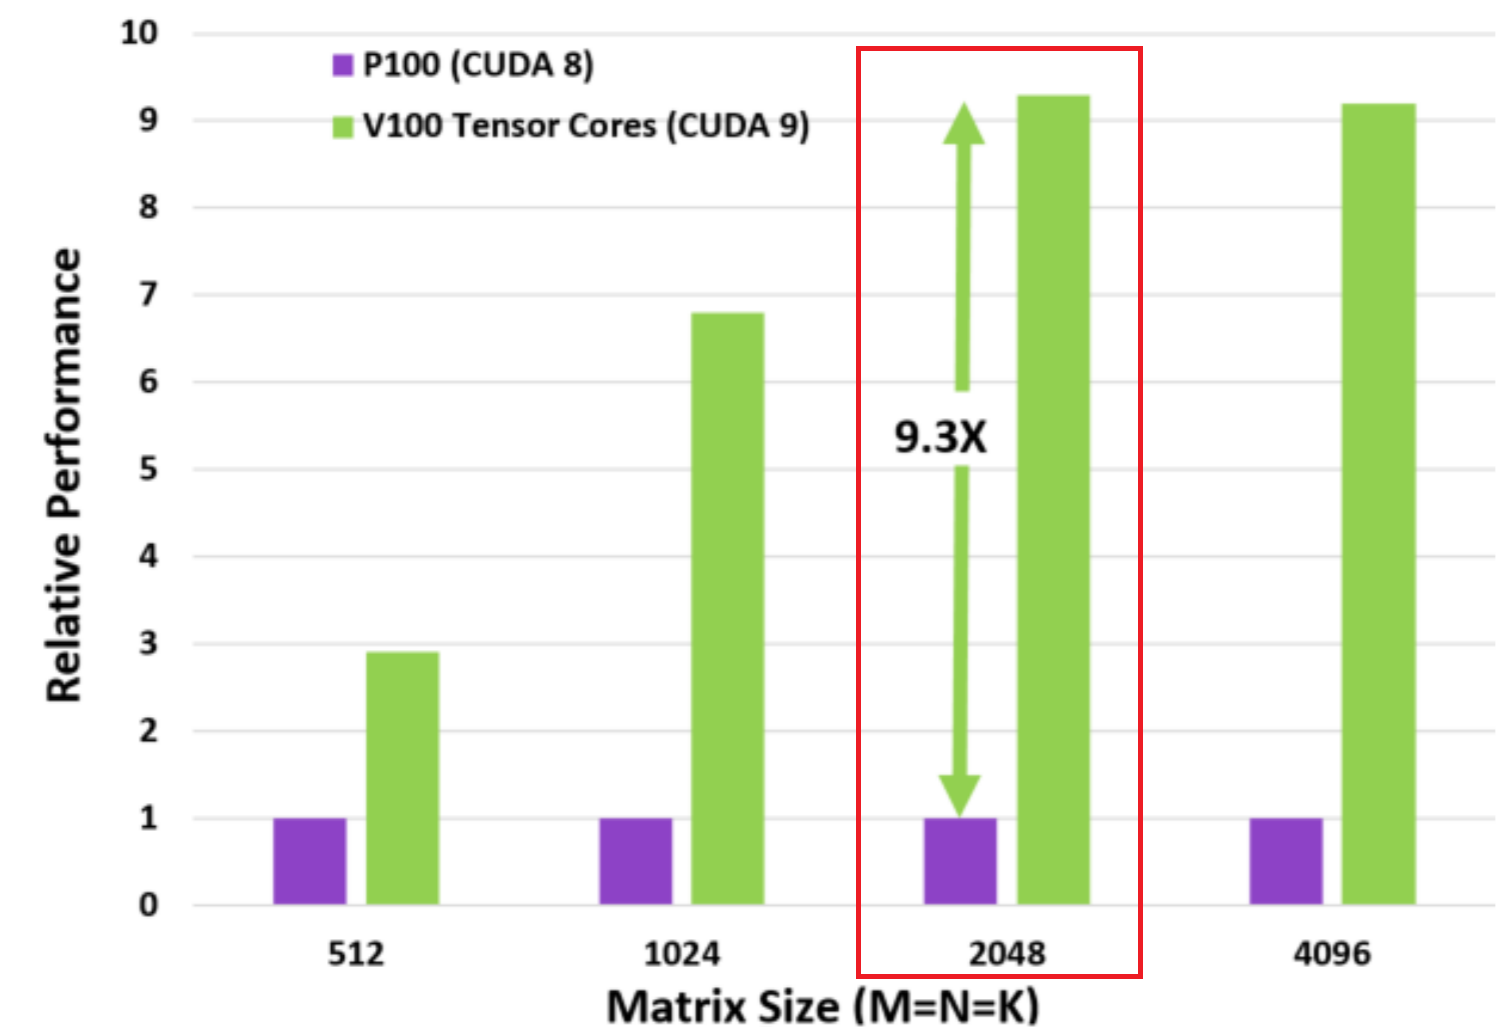
\includegraphics[width=6cm]{figures/VoltaGemmPerf.jpg}
				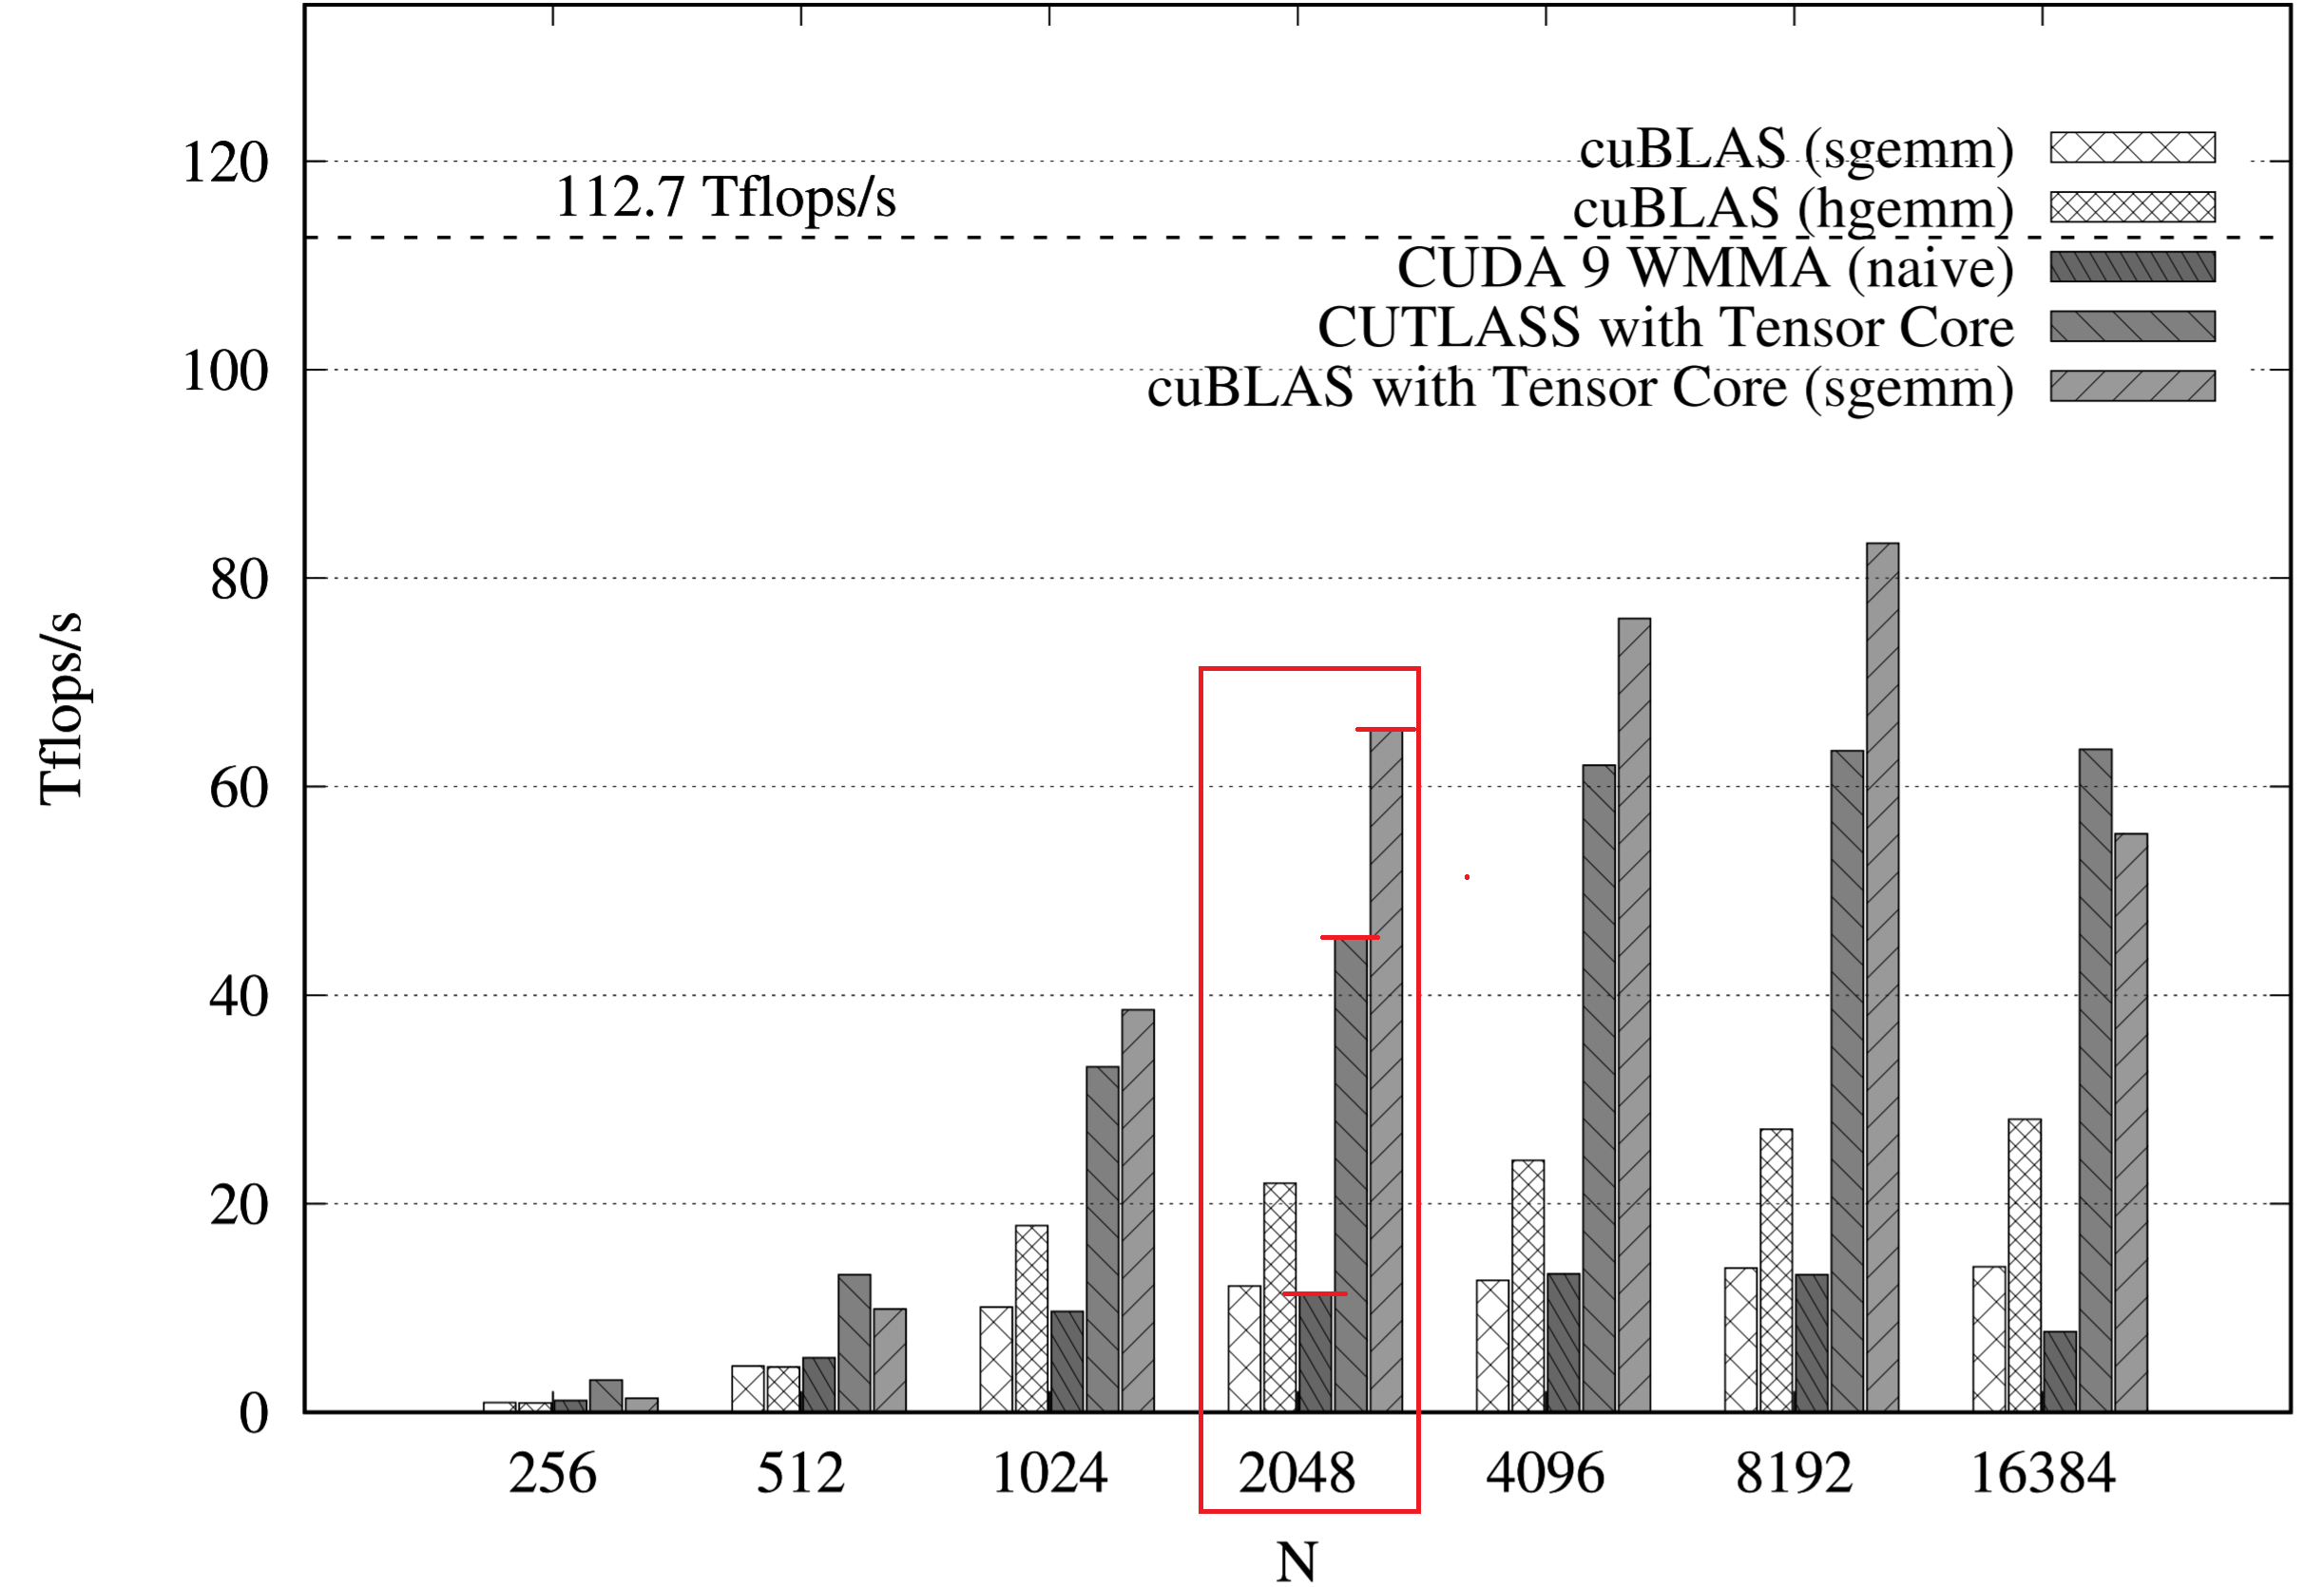
\includegraphics[width=6cm]{figures/ActualGemmPerf.jpg}
				\caption{官方白皮书性能与实际研究中性能比较}\label{Fig.COMPARE}
			\end{figure}
		\end{itemize}
	\end{frame}
	\begin{frame}
		\frametitle{简介}
		\begin{itemize}
			\item 在实际使用框架如Tensor Flow搭建的模型中提升幅度更低。在特定结构的网络中开启张量核心仅能带来60\%-80\%的提升。
			\item {\bf 本文将从Python源码、CUDA C源码、PTX中间代码、SASS硬件代码的层面,借助卷积神经网络和支持向量机这两种经典的应用,对新架构GPU为机器学习应用带来的性能提升进行评估,尝试在代码层面进行优化,并提出设想。}
			\item 具体评估的应用遵循自底向上的结构:
				\begin{itemize}
					\item Benchmark样例(矩阵乘法、\textbf{矩阵乘加}、卷积运算)
					\item 基于CUDA源码的应用(卷积神经网络、支持向量机)
					\item 基于Tensor Flow的应用(卷积神经网络)
				\end{itemize}
			\item 除训练过程外,最后使用TensorRT以及Jetson对部署、推理过程进行优化。
		\end{itemize}
	\end{frame}

	\section{背景}
	\begin{frame}
		\frametitle{背景}
		\begin{itemize}
			\item 机器学习与GPU:目前绝大部分机器学习应用都需要GPU进行加速,而NVIDIA GPU长期占据高性能计算的市场。
			\item NVIDIA GPU结构:自上而下分为图形处理器簇(GPC)、纹理处理器簇(TPC)、流多处理器(SM)。流多处理器中有若干种处理单元如整数、浮点、逻辑单元。
			\item 伏特架构/图灵架构:在流处理器中加入了张量核心的新架构,分别对应计算能力7.0与7.5,图灵是消费级芯片,屏蔽了一些硬件。
			\item 张量核心:专为矩阵乘加设计的硬件,以半精度浮点进行运算(FP16),以wmma指令批量执行原先整数点积指令与累加指令执行的任务。
			\item 纹理内存:访问时将二维空间上的周围数据加载进入缓存,其余存储系统为加载一行。
			\item 线程束:内含32个GPU线程,作为基本的调度、同步单元。
			\item 矩阵乘加:通用矩阵乘法,即两矩阵相乘再与偏置累加。大量存在于神经网络计算。
			\item TensorRT与Jetson:TensorRT是一个GPU推理引擎,用于优化训练完毕的模型,加速推理。Jetson是NVIDIA开发的面向嵌入式应用的芯片。
		\end{itemize}
	\end{frame}

	\section{相关工作}
	\begin{frame}
		\frametitle{相关工作}
		\begin{itemize}
			\item GPGPU-SIM:PTX中间代码执行的软件层面模拟。
			\item SMart, PerfSIM:SASS硬件代码执行的软件层面模拟以及RTL仿真。
			\item ThunderSVM:并行支持向量机。
			\item Leng J.:大型集群的性能、能耗优化。
			\item Mahmoud K.:访存优化
			\item ?张量核心
		\end{itemize}
	\end{frame}

	\section{实验平台}
	\begin{frame}
		\frametitle{实验平台}
		\begin{table}
			\centering
			\caption{实验平台}
			\begin{tabular}{cc}
				\toprule
				项目	&	内容\\
				\midrule
				CPU		&	AMD Ryzen ThreadRipper 2990WX 32C64T @ 3.0GHz\\
				主板		&	MSI X399\\
				内存		&	CORSAIR DDR4 3200 @ 16-15-15-15-34-1T 128GB\\
				GPU		&	NVIDIA Geforce RTX 2080TI (Turing)\\
				硬盘		&	INTEL750 NVMe PCIe 1.2TB * 2 @ RAID 0\\
				系统		&	Windows 10 64-bit build 17763\\	
				CUDA	&	Ver. 10.1, 10.0, 9.2, 9.0\\
				CUTLASS & Ver. 1.2, 1.3\\
				其他		&	Jetson TX2 $ * $\\
				\bottomrule
			\end{tabular}
		\end{table}
	\end{frame}
	
	\section{实验内容}
	\subsection{Benchmark}
	\subsubsection{矩阵乘加}
	\begin{frame}
		\frametitle{Benchmark::矩阵乘加}
		由于新老架构GPU在参数、外围设备等方面均有改进,为了重点研究张量核心的性能,本文中的实验均在RTX 2080TI上通过开启/关闭张量核心进行评估。
		\begin{figure}
			\centering
			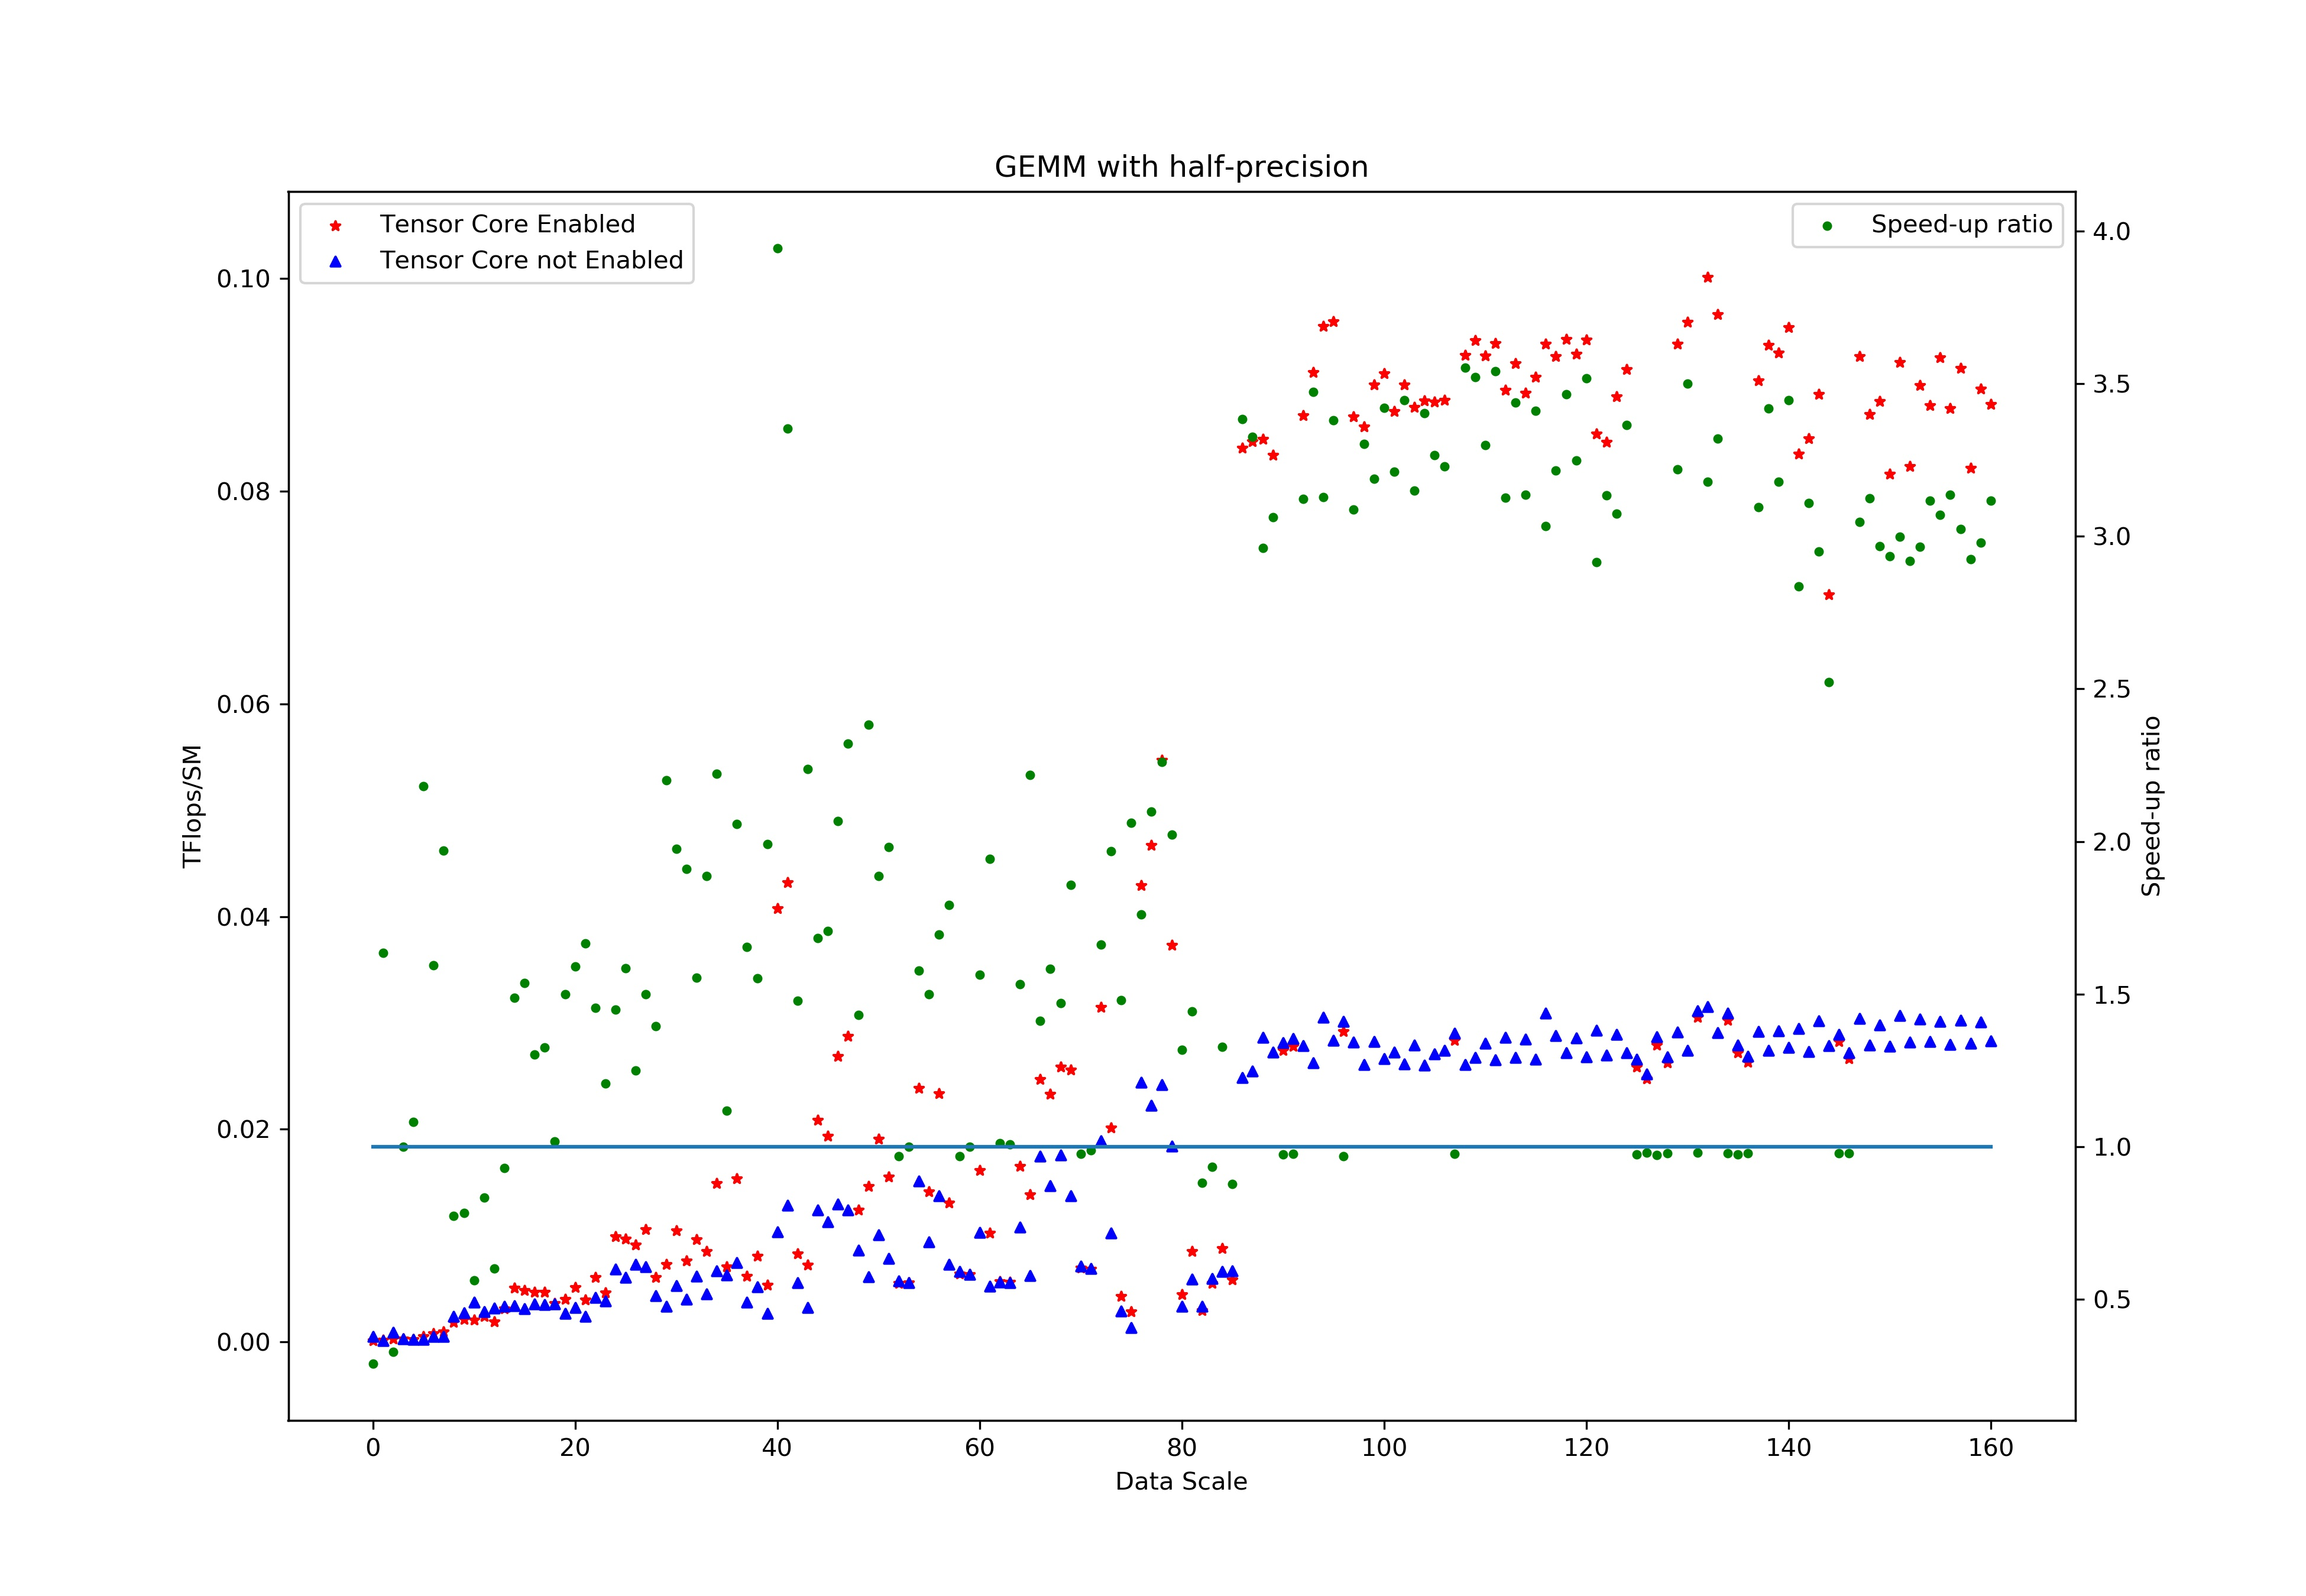
\includegraphics[width=5.5cm]{figures/GEMM-Half-TF.jpg}
			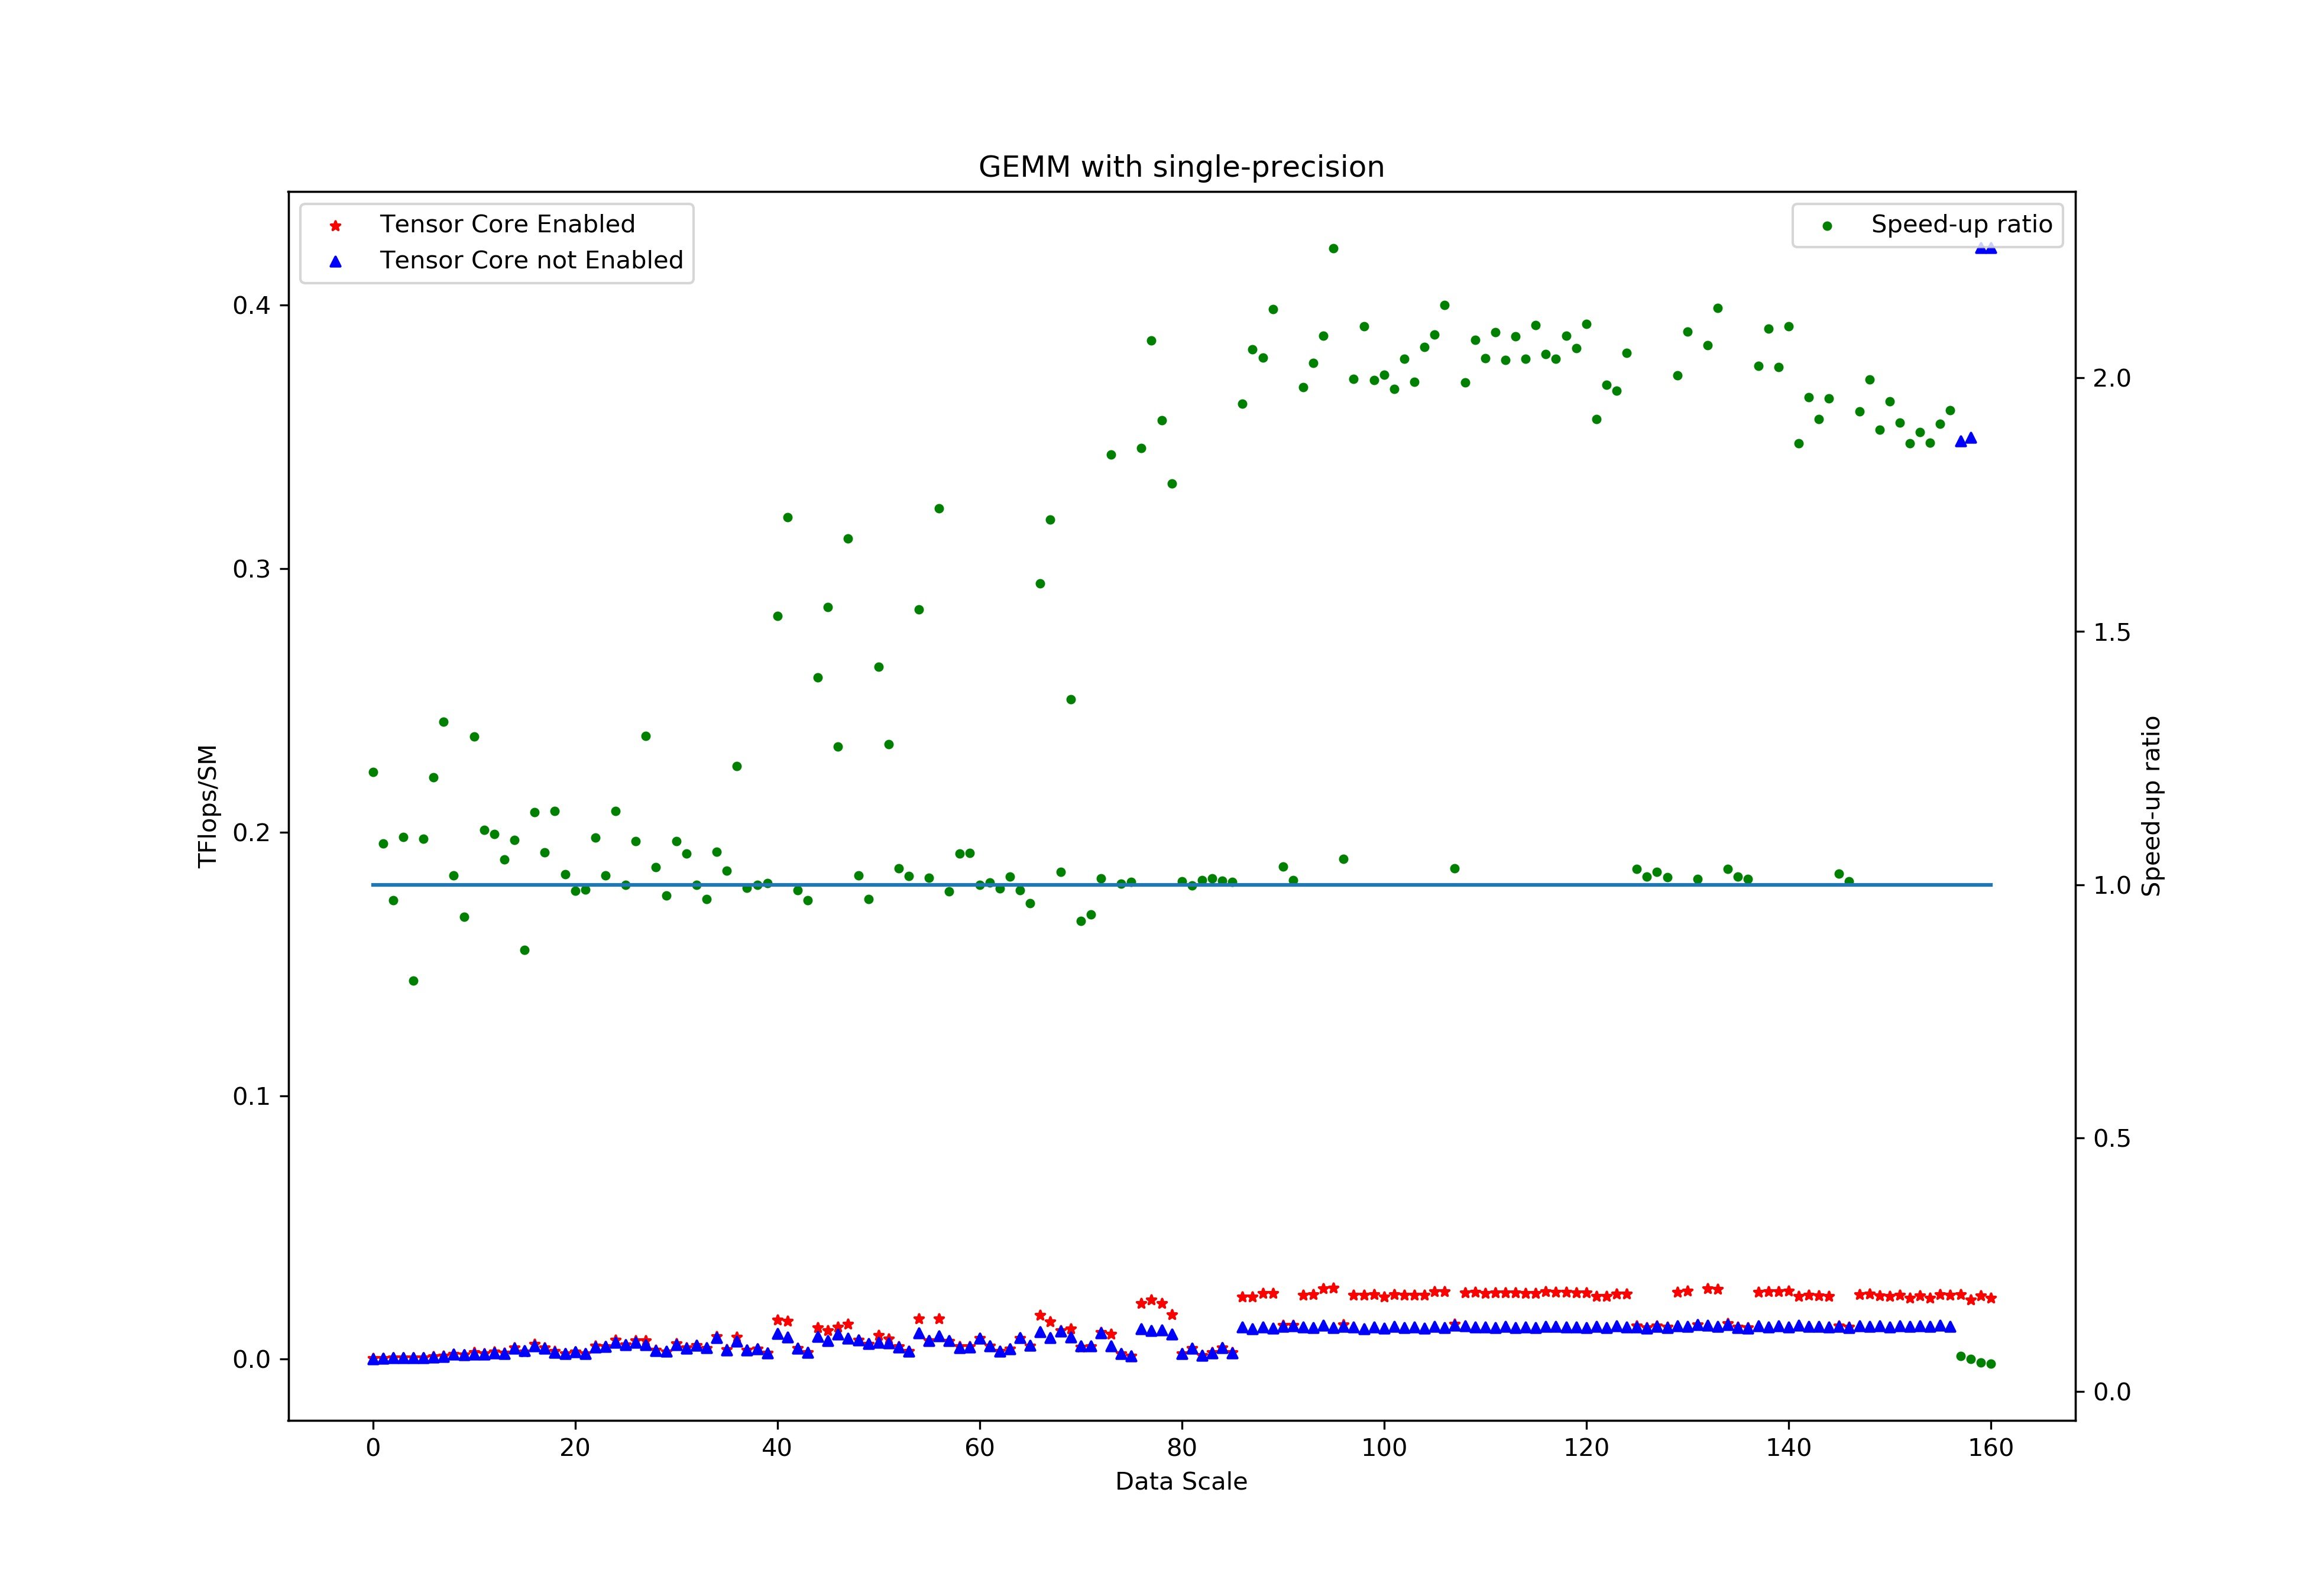
\includegraphics[width=5.5cm]{figures/GEMM-Single-TF.jpg}
			\caption{不同计算量下开启和关闭张量核心的性能(半精度/单精度)}\label{Fig.GEMM}
		\end{figure}
		在计算量较大的情况下,开启张量核心后半精度性能提升3-4倍,单精度性能提升2倍。
	\end{frame}
	
	\begin{frame}
		\frametitle{Benchmark::矩阵乘加}
		使用nvprof和NSight进行分析:
		\begin{table}
			\centering
			\caption{开启/关闭张量核心的对比}
			\begin{tabular}{ccc}
				\toprule
				项目	&	开启张量核心 & 关闭张量核心\\
				
				\midrule
				CUDA设备同步耗时 & \textbf{186.15s} & 543.51\\
				CUDA设备同步耗时占比 & \textbf{79.29\%} & 91.40\%\\
				一次乘加所需计算指令 & \textbf{一条wmma} & 若干条idp/idp4a+累加指令\\
				每条计算指令延迟 & \textbf{wmma: 8时钟周期} & idp/idp4a: 4时钟周期\\
				上下文切换时间占比 & \textbf{44.39\%} & 52.52\%\\
				\bottomrule
			\end{tabular}
		\end{table}
		开启张量核心后设备同步、上下文切换等死时间减少,原因为张量核心整合多次计算为一次。并行可扩展性强(更大规模的MMA)(\textbf{进一步扩大矩阵乘加指令的规模})。结果中可见设备同步耗时仍然很长,目前CUDA仅支持线程束级别的同步,导致频繁的同步(更细粒度的线程同步机制)。
	\end{frame}

	\begin{frame}
		\frametitle{Benchmark::矩阵乘加}
		根据官方文档说明,张量核心对于矩阵裁切形状较为敏感,故将实验结果按加速比排序并按形状特征着色,形状特征分为:能够被32整除、能够被8整除,无法被整除。
		\begin{figure}
			\centering
			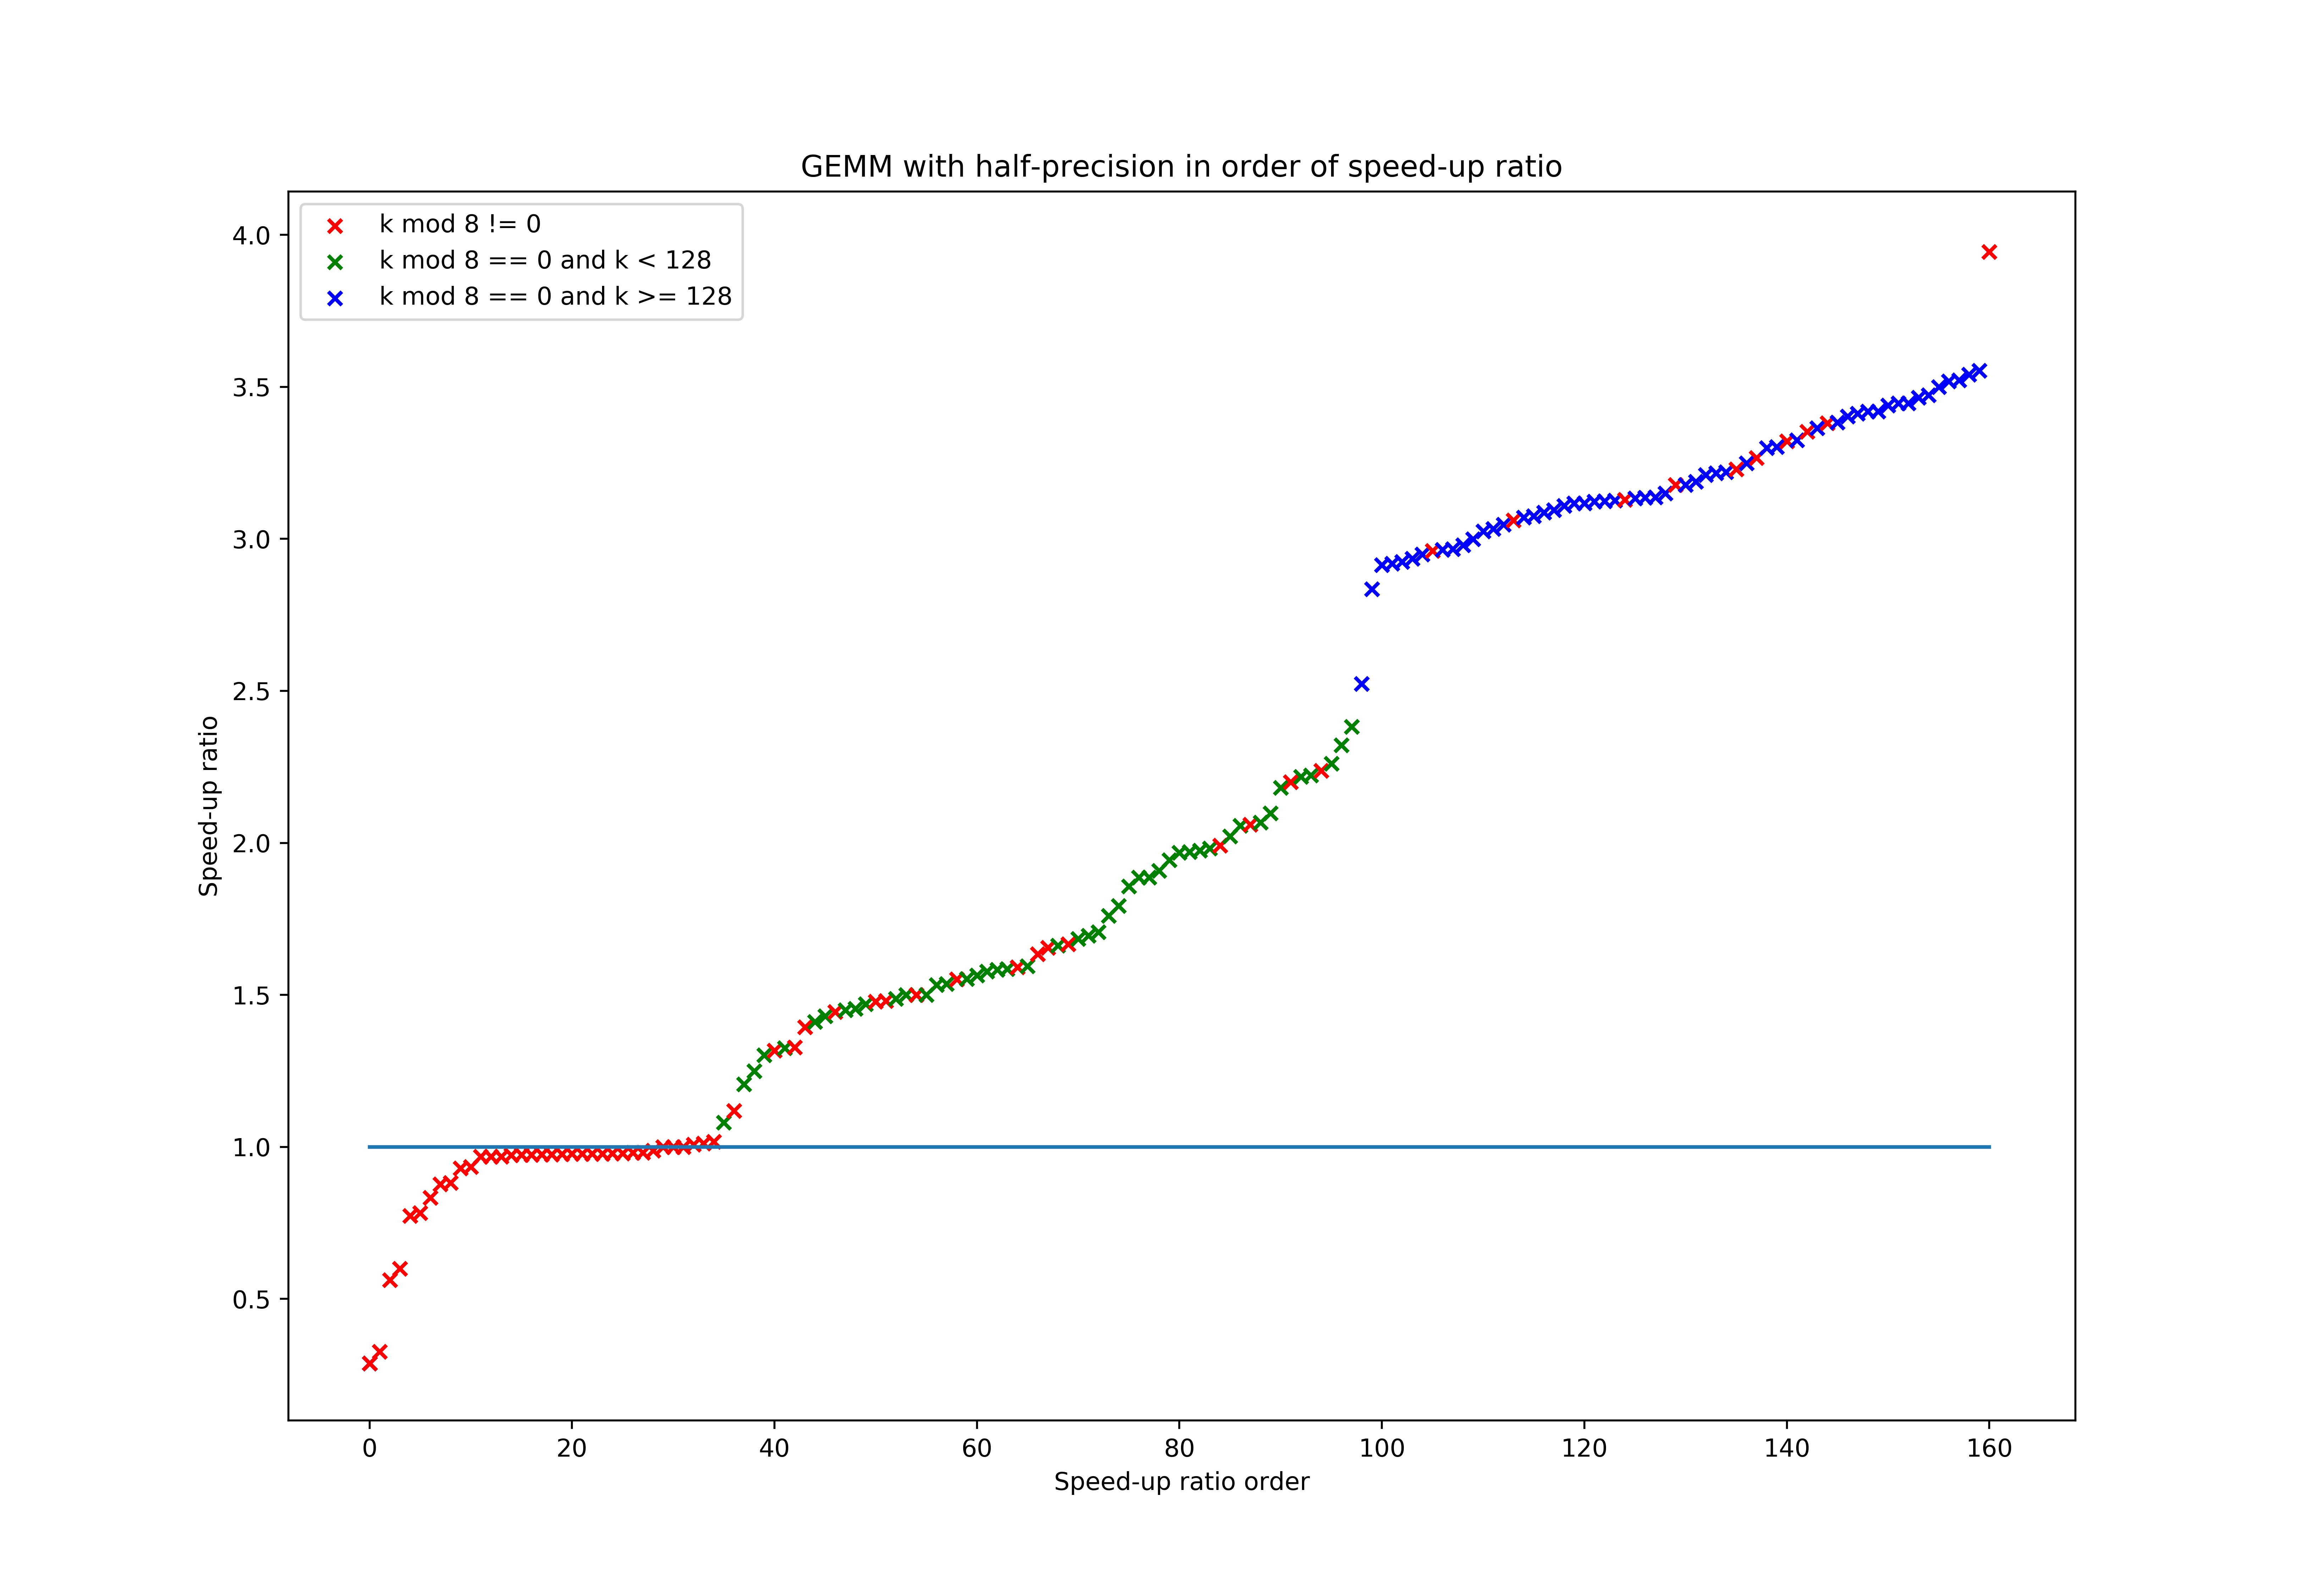
\includegraphics[width=5.5cm]{figures/GEMM-Half-TF-Byratio-Tri.jpg}
			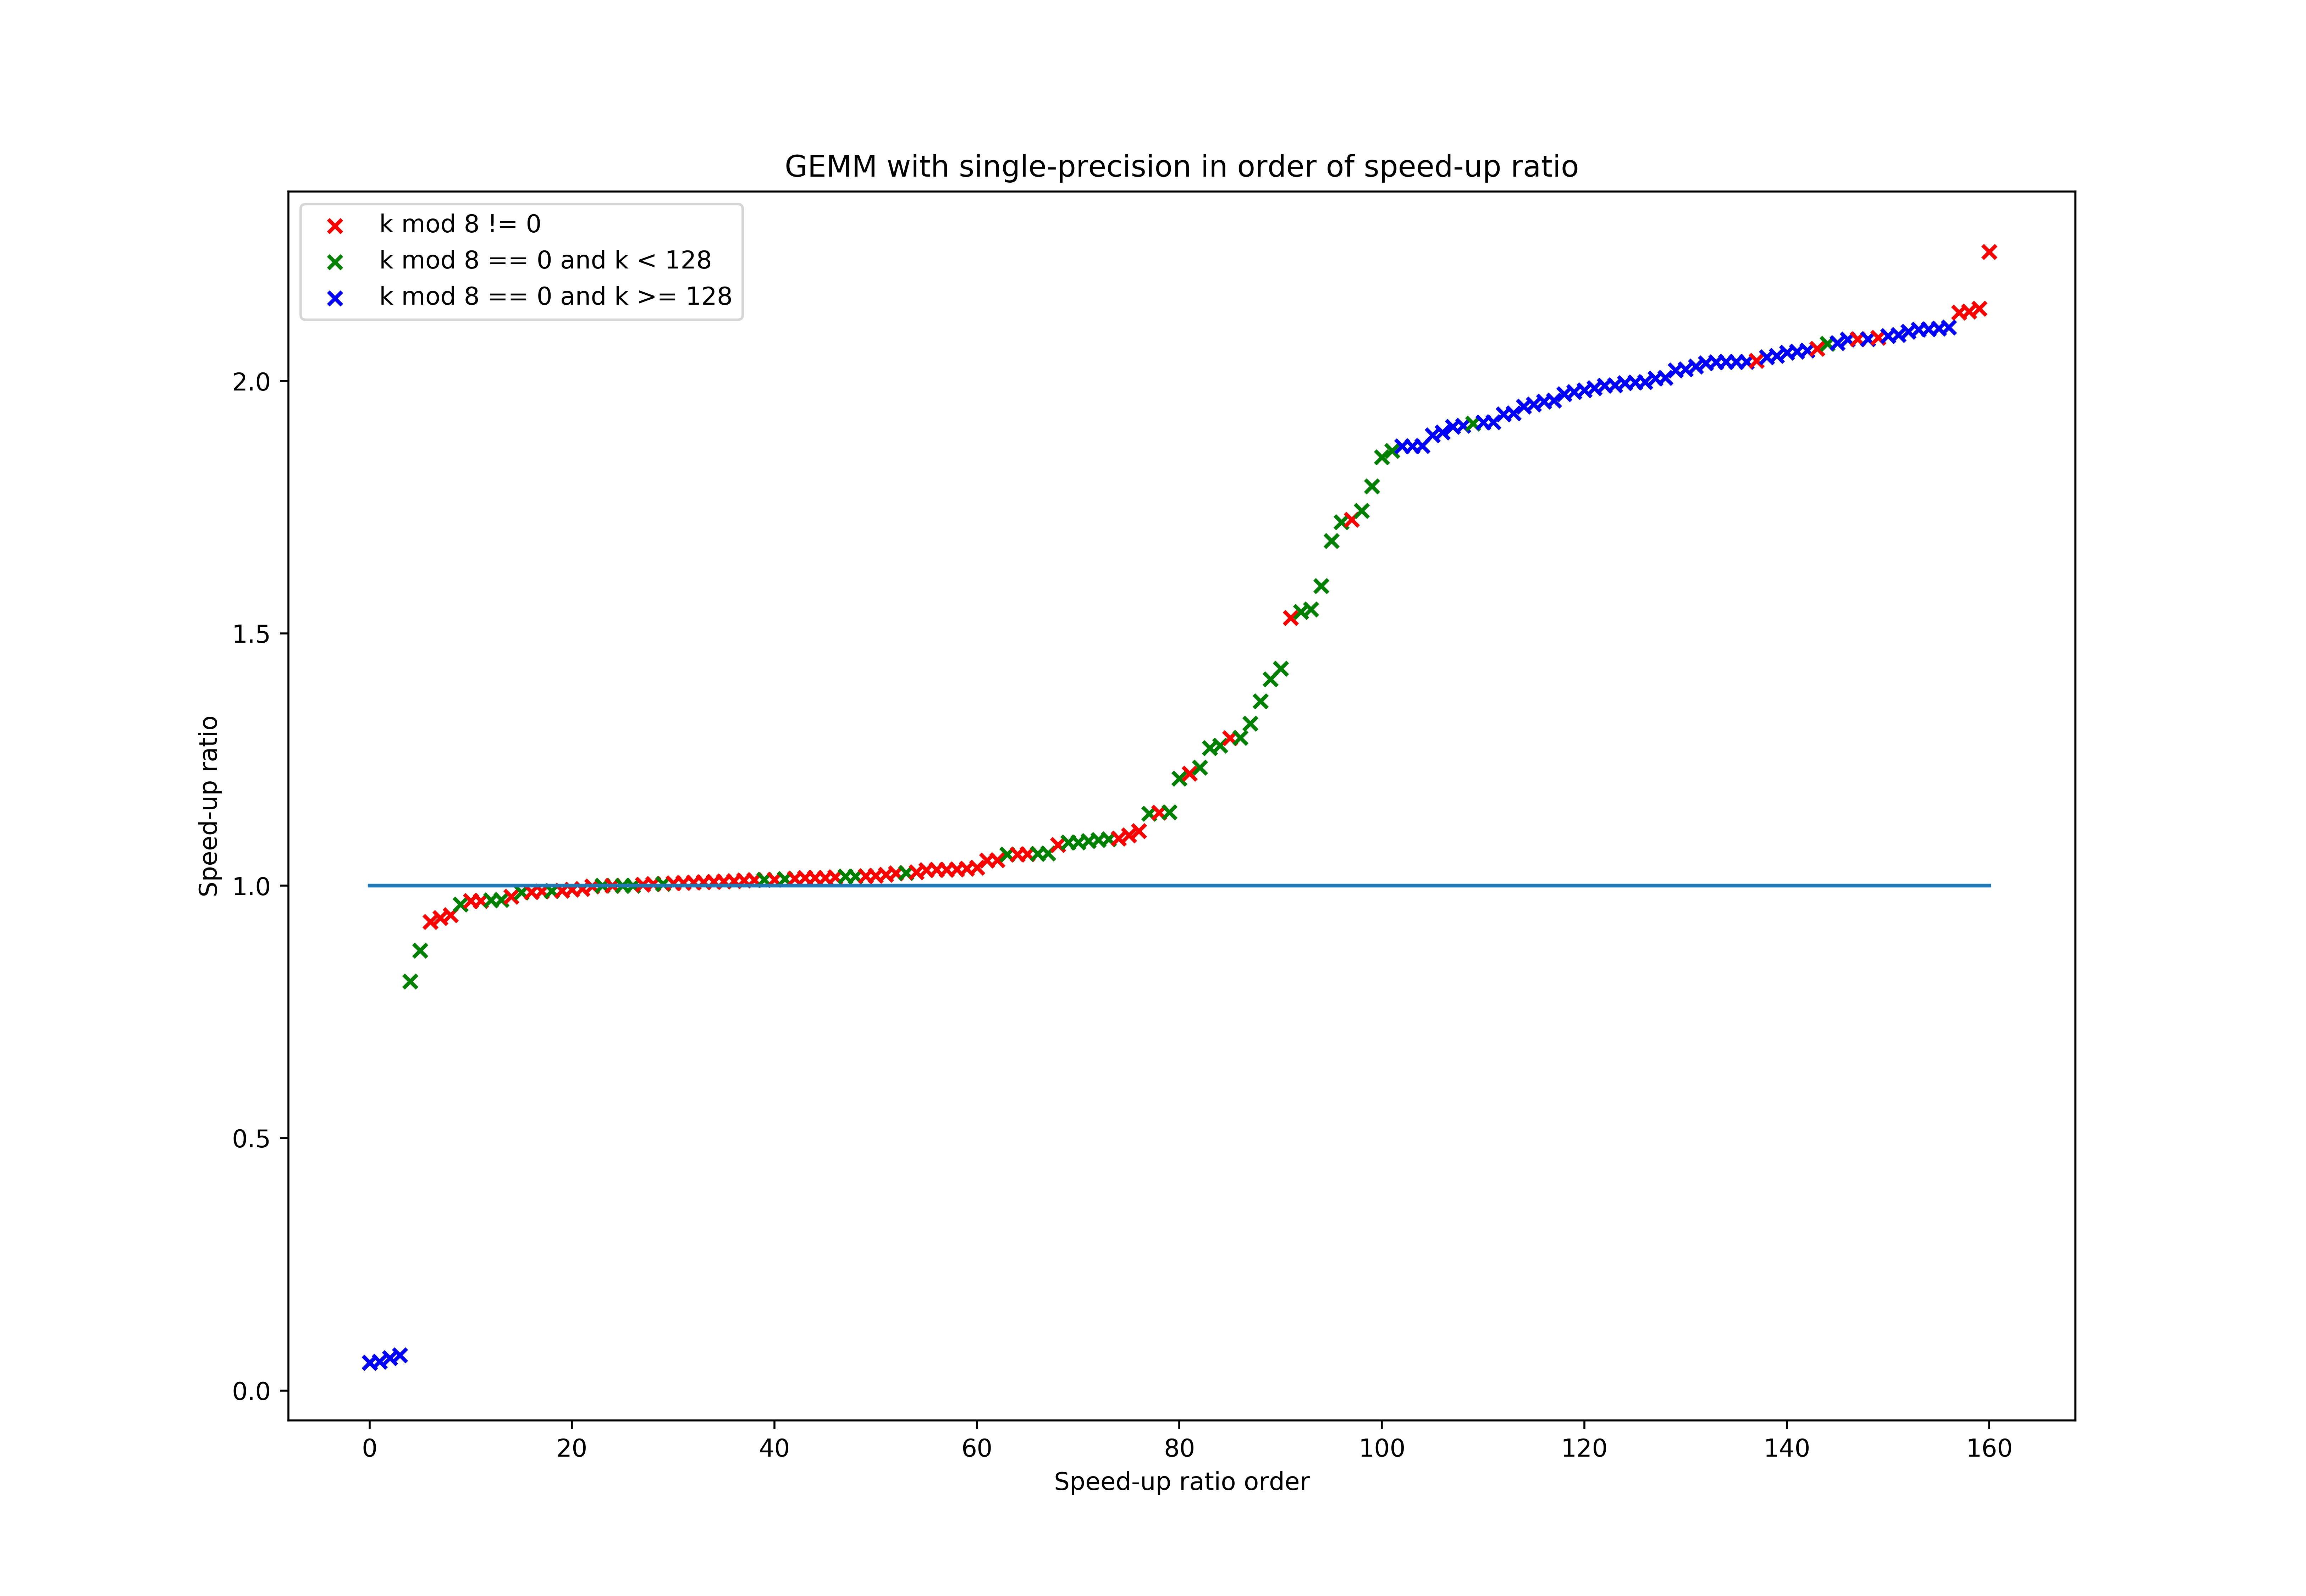
\includegraphics[width=5.5cm]{figures/GEMM-Single-TF-Byratio-Tri.jpg}
			\caption{不同计算量下开启和关闭张量核心的性能(半精度/单精度)-按加速比排序并着色}\label{Fig.GEMMRATIO}
		\end{figure}
		可见,当矩阵三维中K维度为32的整数倍时性能提升幅度最大,实际使用时,应对其数据规模、超参数进行优化以确保最大提升幅度。
	\end{frame}

	\subsubsection{矩阵乘法}
	\begin{frame}
		\frametitle{Benchmark::矩阵乘法}
		在使用矩阵乘加评估GPU性能前,业内采用矩阵乘法对GPU在机器学习中的性能进行评估。本文考察使用CUDA中cuBLAS提供的API,以及不使用API自行实现矩阵乘法的方法下矩阵乘法的性能。可见自行实现矩阵乘法性能极低,应尽量使用API完成基本的计算。
		\begin{figure}
			\centering
			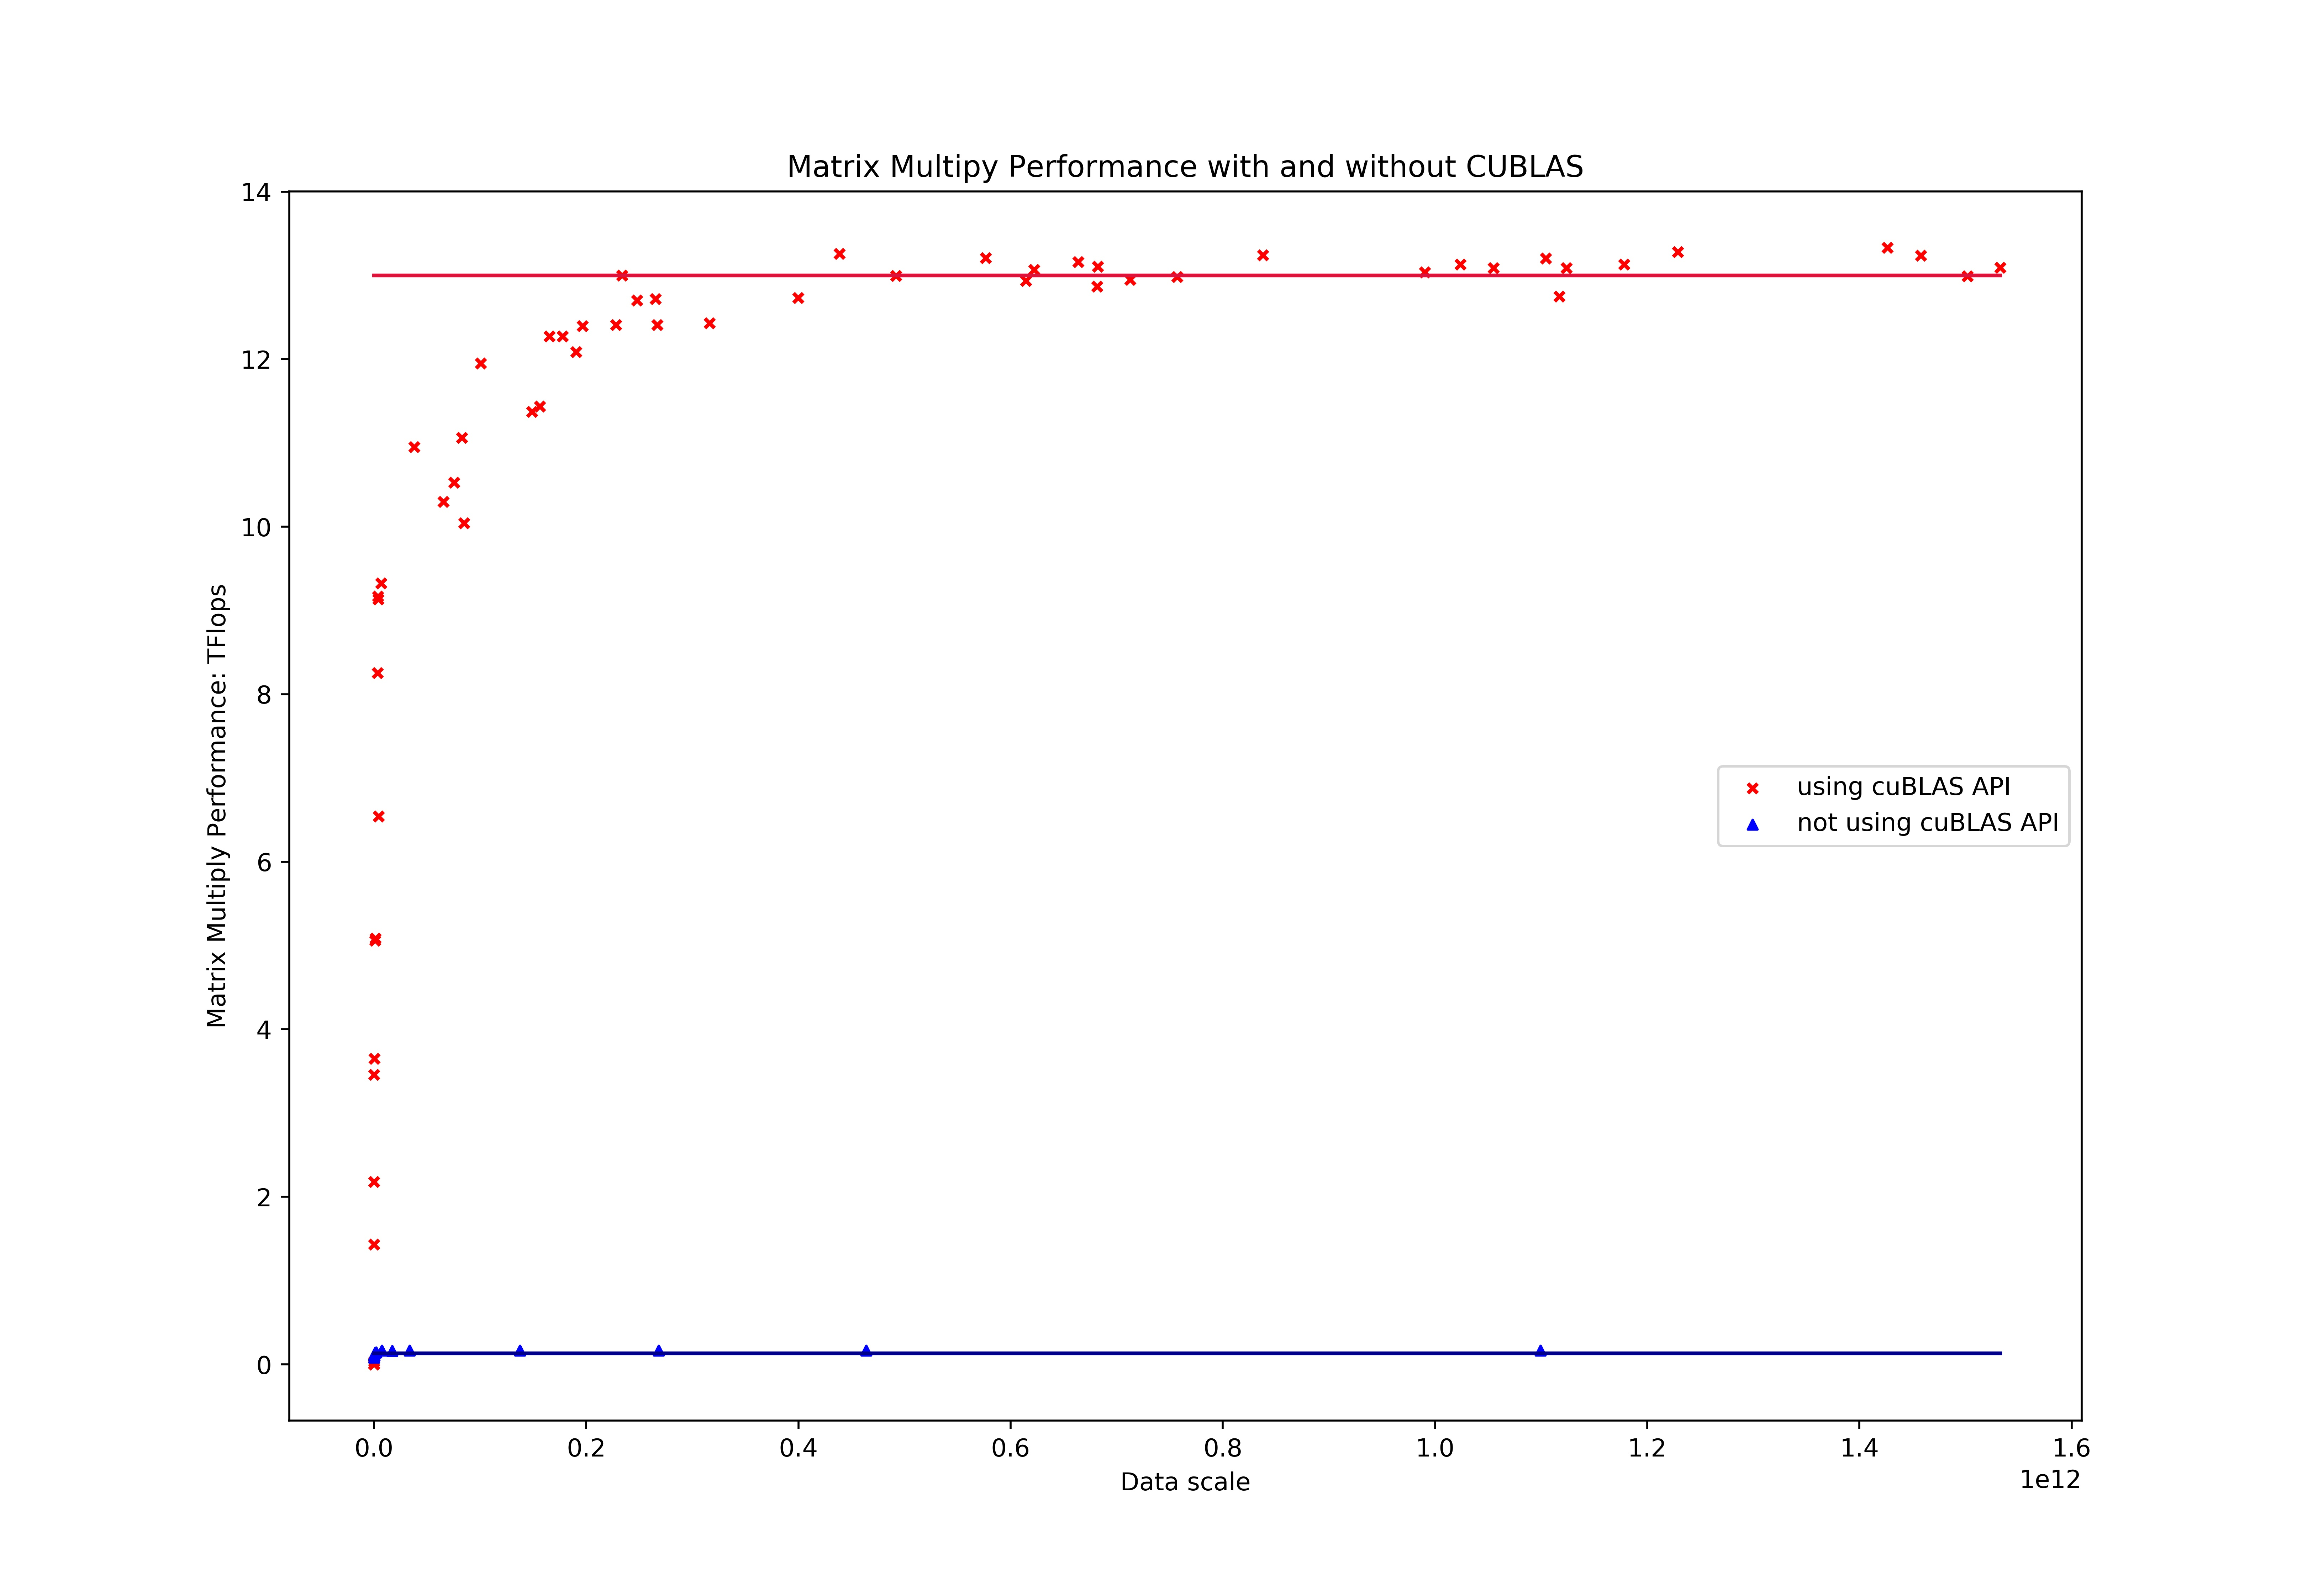
\includegraphics[width=7cm]{figures/CUBLASPerf.jpg}
			\caption{使用和不使用cuBLAS库的单精度矩阵乘法性能}\label{Fig.MM}
		\end{figure}
		
	\end{frame}
	\subsubsection{卷积}
	\begin{frame}
		\frametitle{Benchmark::卷积}
		卷积大量存在于神经网络、图像处理计算中,本节评估如下几种卷积计算方式,这些方式分别具有各自特点。
		\begin{table}
			\centering
			\caption{卷积计算方式及特征}
			\begin{tabular}{cc}
				\toprule
				卷积计算方式	&	描述\\
				\midrule
				基于FFT的CUDA内建卷积 & 使用CUDA提供的基于FFT的卷积库\\
				基于FFT的自定义卷积 & 使用CUDA提供的FFT库实现卷积\\
				基于矩阵乘加的CUDA内建卷积 & 使用CUDA提供的利用张量核心的API\\
				直接卷积(全局内存) & 直接计算每一个单元的值,基于全局内存\\
				直接卷积(纹理内存) & 直接计算每一个单元的值,基于纹理内存\\
				\bottomrule
			\end{tabular}
		\end{table}
	\end{frame}

	\begin{frame}
		\frametitle{Benchmark::卷积}
		结果中大尺寸图像与小尺寸图像差异较大。
		\begin{figure}
			\centering
			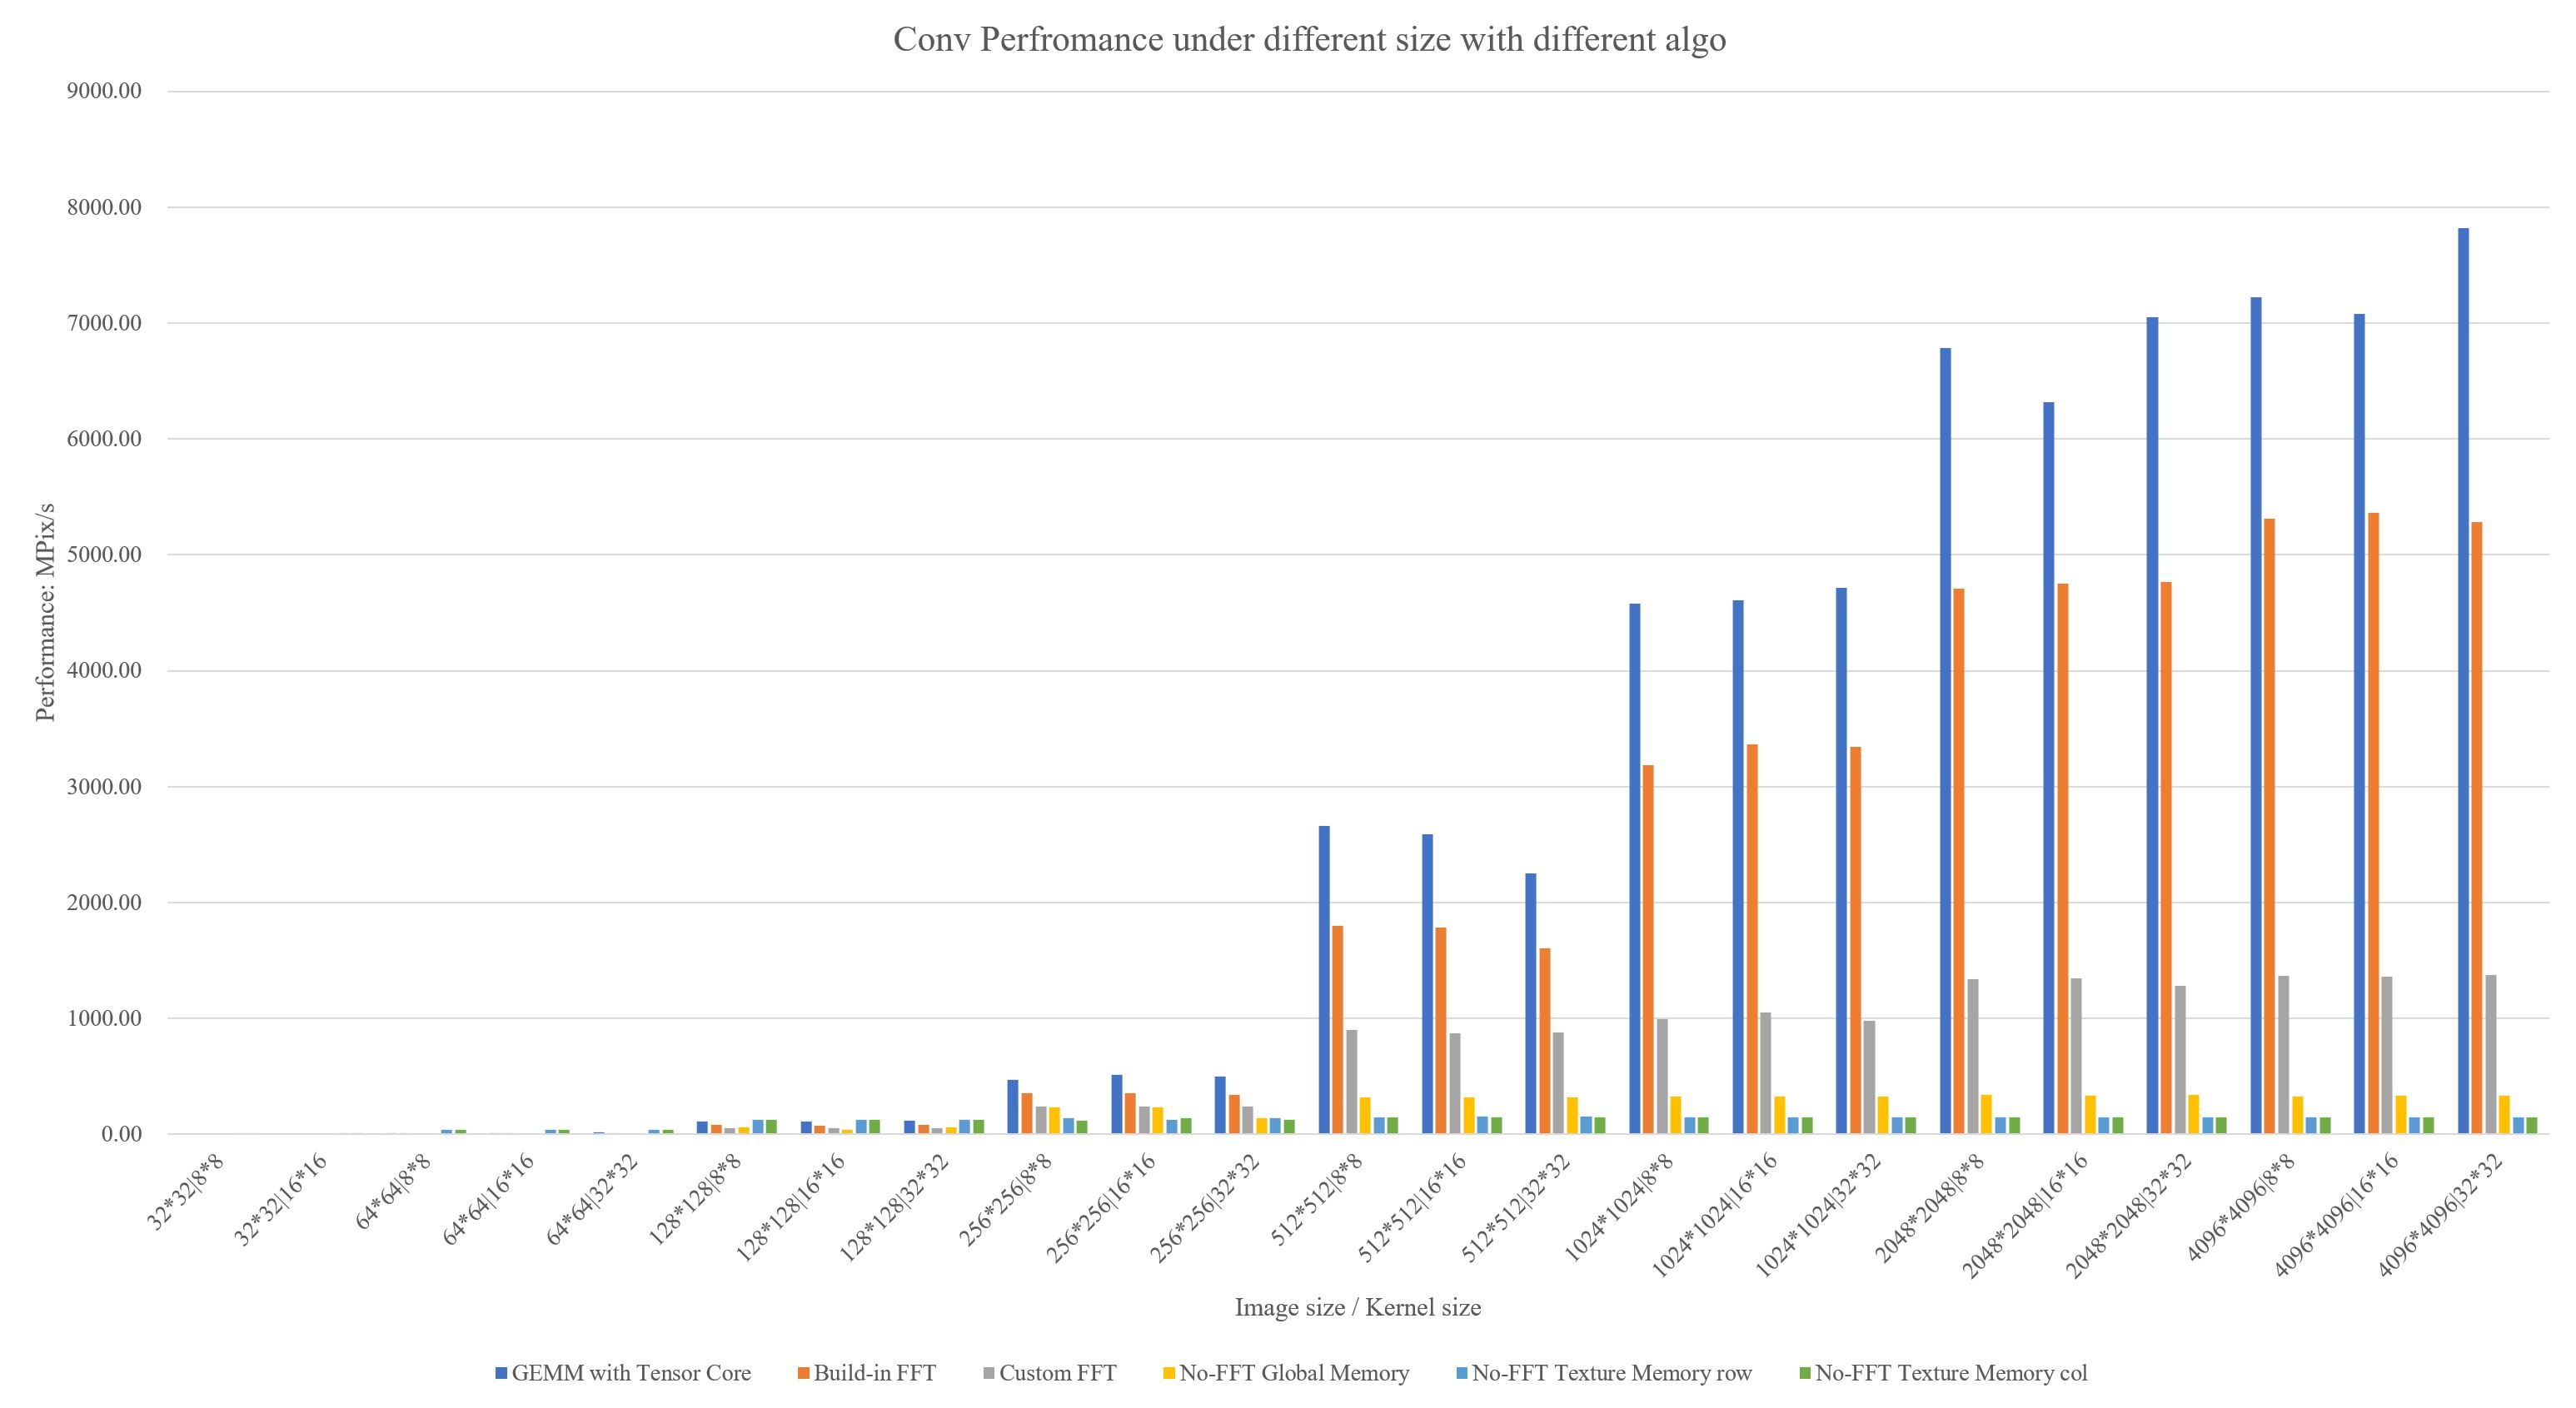
\includegraphics[width=6.5cm]{figures/CONVPerf.jpg}
			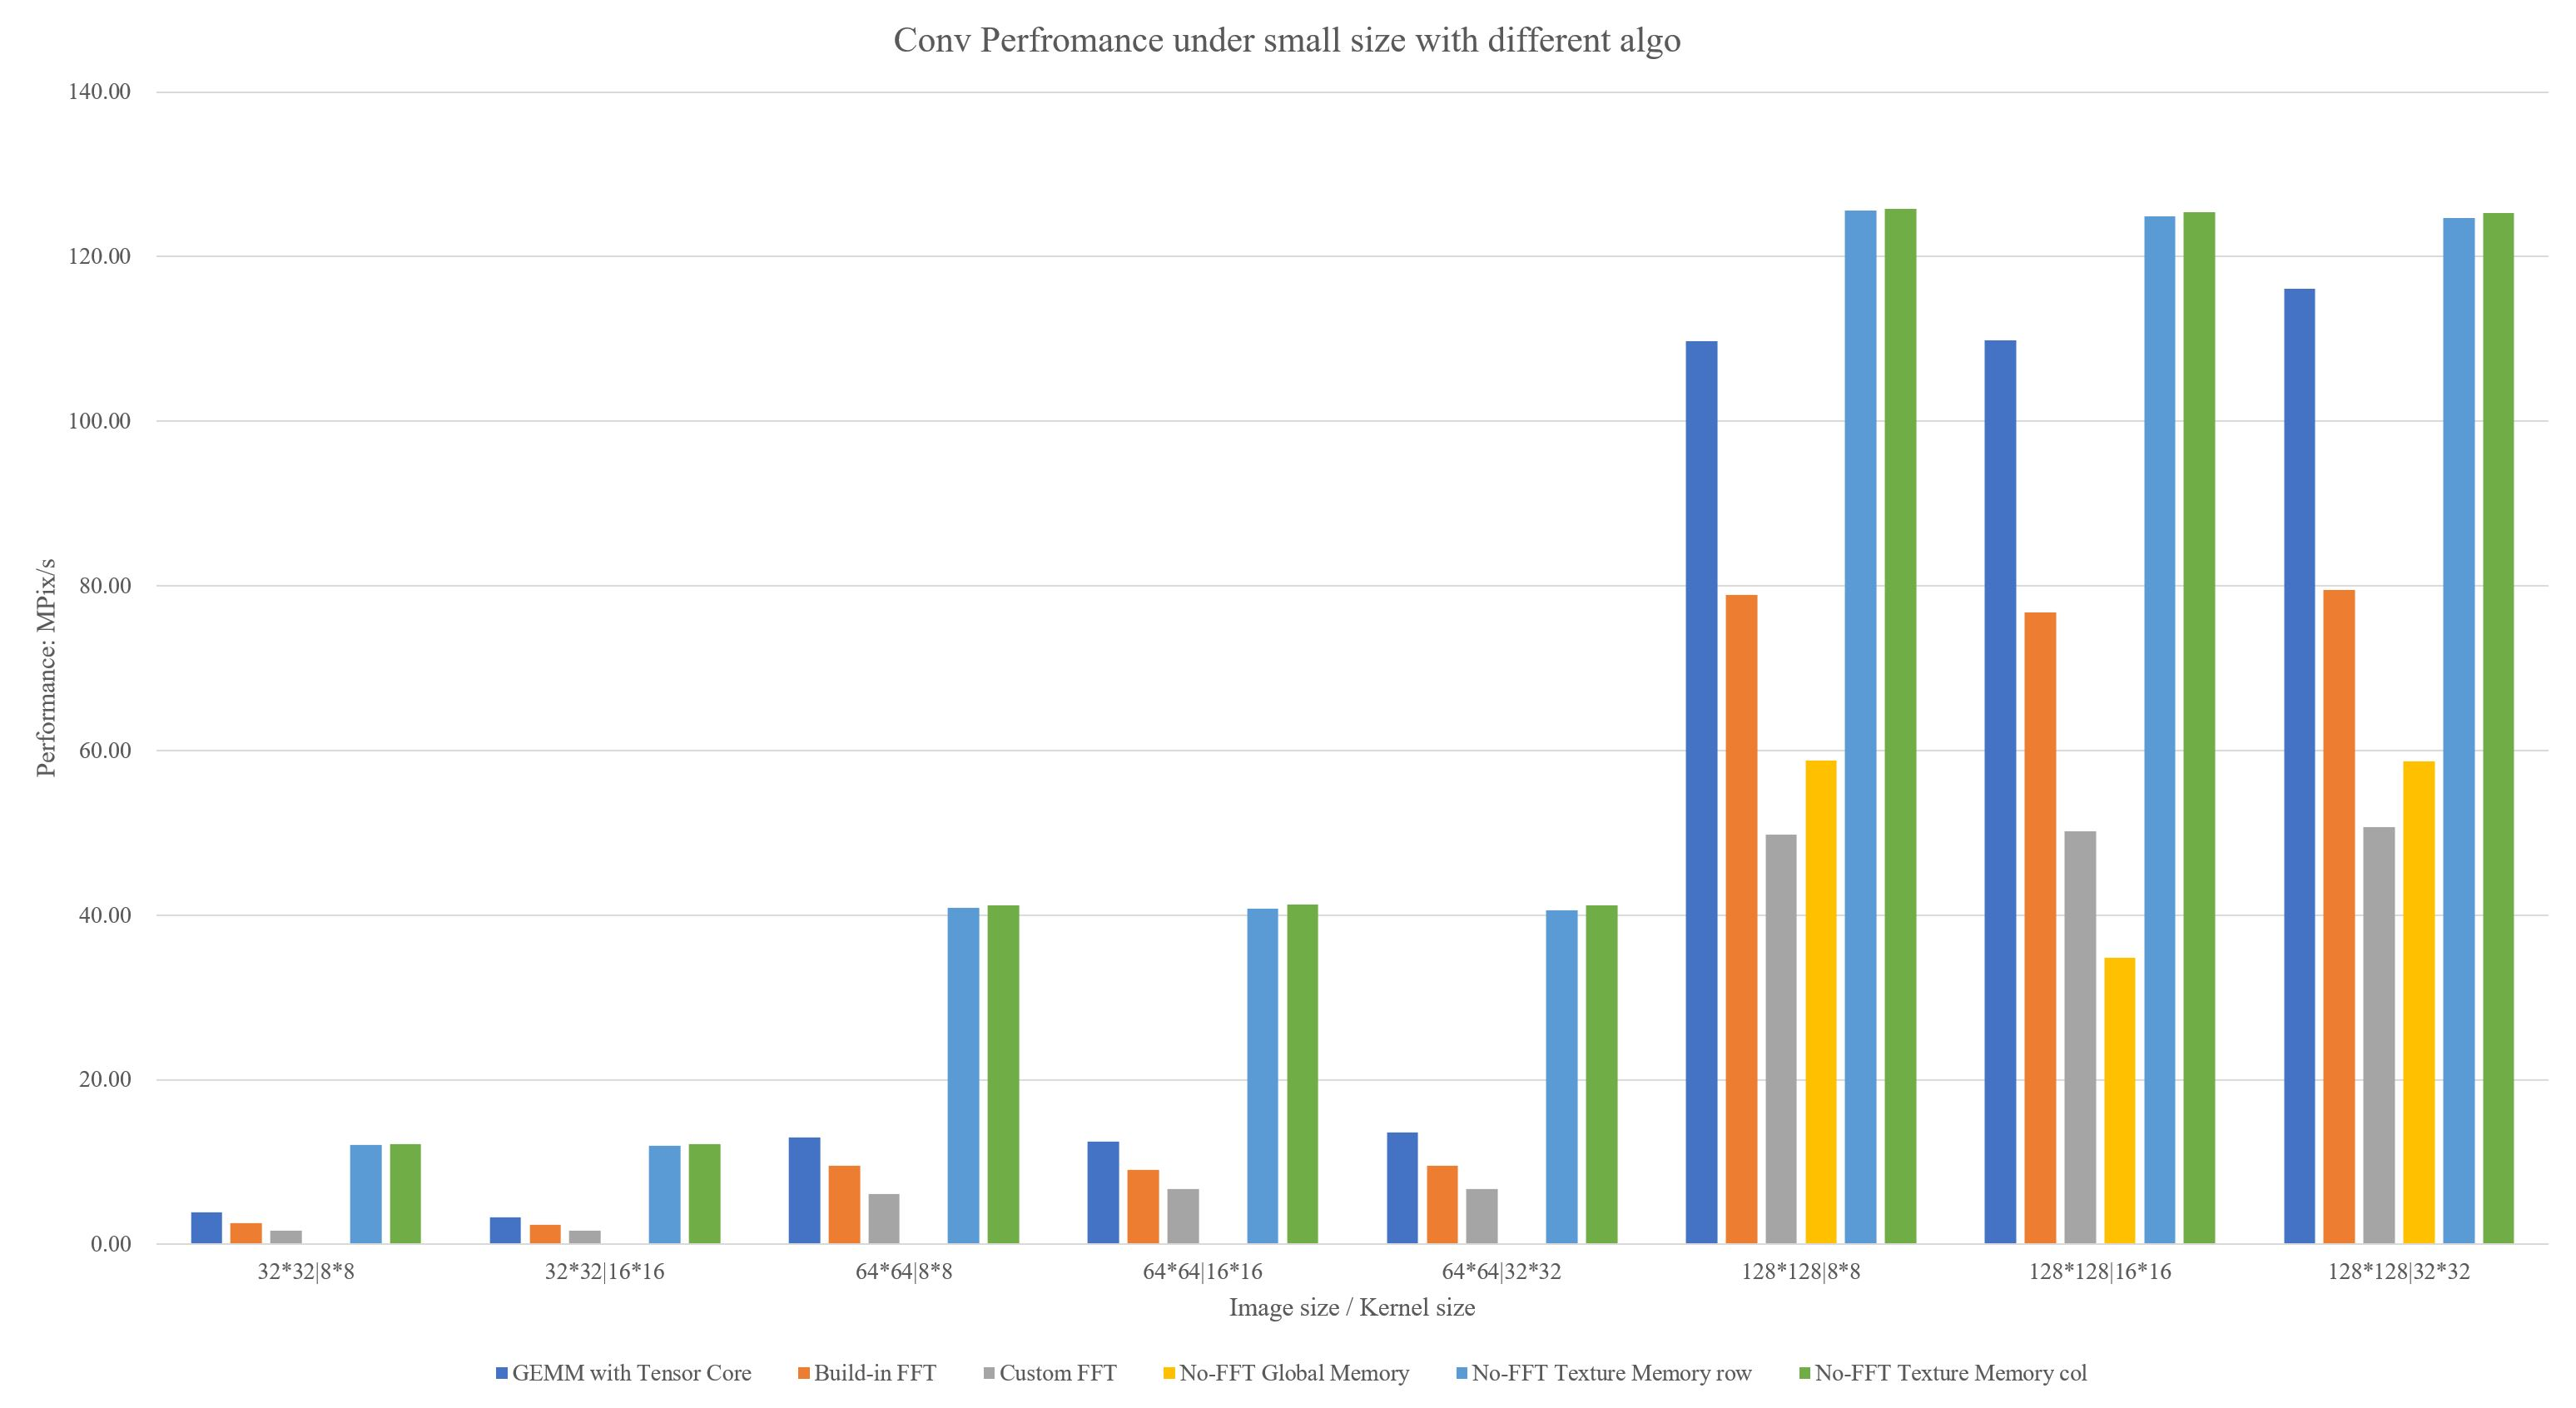
\includegraphics[width=6.5cm]{figures/CONVSubPerf.jpg}
			\caption{不同方法的卷积计算性能(大尺寸图像/小尺寸图像)}\label{Fig.CONV}
		\end{figure}
		大尺寸图像下基于GEMM的方法优势明显,小尺寸图像下基于纹理内存的方法优势明显。
	\end{frame}

	\begin{frame}
		\frametitle{Benchamrk::卷积}
		使用nvprof和NSight进行分析:可见对于GEMM,主要瓶颈在于访存。而对于纹理内存的直接方式,主要瓶颈在于计算本身。
		\begin{table}
			\centering
			\caption{快速傅里叶变换/纹理内存直接方式计算卷积的对比}
			\begin{tabular}{cclcc}
				\toprule
				类型 & 计算方法 & 项目 & 小尺寸用时占比 & 大尺寸用时占比\\
				\midrule
				GPU 活动& FFT & 内存复制 & 8.78\% & 62.91\%\\
				&				&  计算 & 16.88\% & 4.25\%\\
				& 直接(纹理)&  内存复制 & 0.46\% & 1.88\%\\
				&				&  计算 & 99.19\% & 98.12\%\\
				\midrule
				API 调用 &FFT &内存分配、释放 &99.09\% & 96.09\% \\
				&				& 设备同步 &0.12\% & 1.30\%\\
				&直接(纹理)& 内存分配、释放 & 77.65\% & 33.69\%\\
				&				& 设备同步 & 1.00\% & 55.01\% \\
				&			    & 上下文切换 & 19.51\% & 9.39\%\\
				\bottomrule
			\end{tabular} \label{table-CONVPROF} 
		\end{table}
	\end{frame}
	\subsection{CUDA}
	\subsubsection{卷积神经网络(cuDNN)}
	\begin{frame}
		\frametitle{CUDA C::卷积神经网络}
		完整的卷积神经网络涉及三部分,如表所示。本文将考察开启和关闭张量核心下三部分的性能变化。
		\begin{table}
			\centering
			\caption{卷积神经网络中三部分计算任务及特征}
			\begin{tabular}{ccc}
				\toprule
				过程 & cuDNN::cuDNNConvolution-	&	描述\\
				\midrule
				前向传播 & Forward() & 包含大量卷积、混合矩阵运算 \\
				反向传播更新卷积核权重 & BackwardFilter() & 包含大量梯度、浮点数值计算,涉及卷积运算\\
				反向传播更新连接权重 & BackwardData() & 包含大量梯度、浮点数值计算\\
				\bottomrule
			\end{tabular} 
		\end{table}
	\end{frame}

	\begin{frame}
		\frametitle{CUDA C::卷积神经网络}
		\begin{figure}
			\centering
			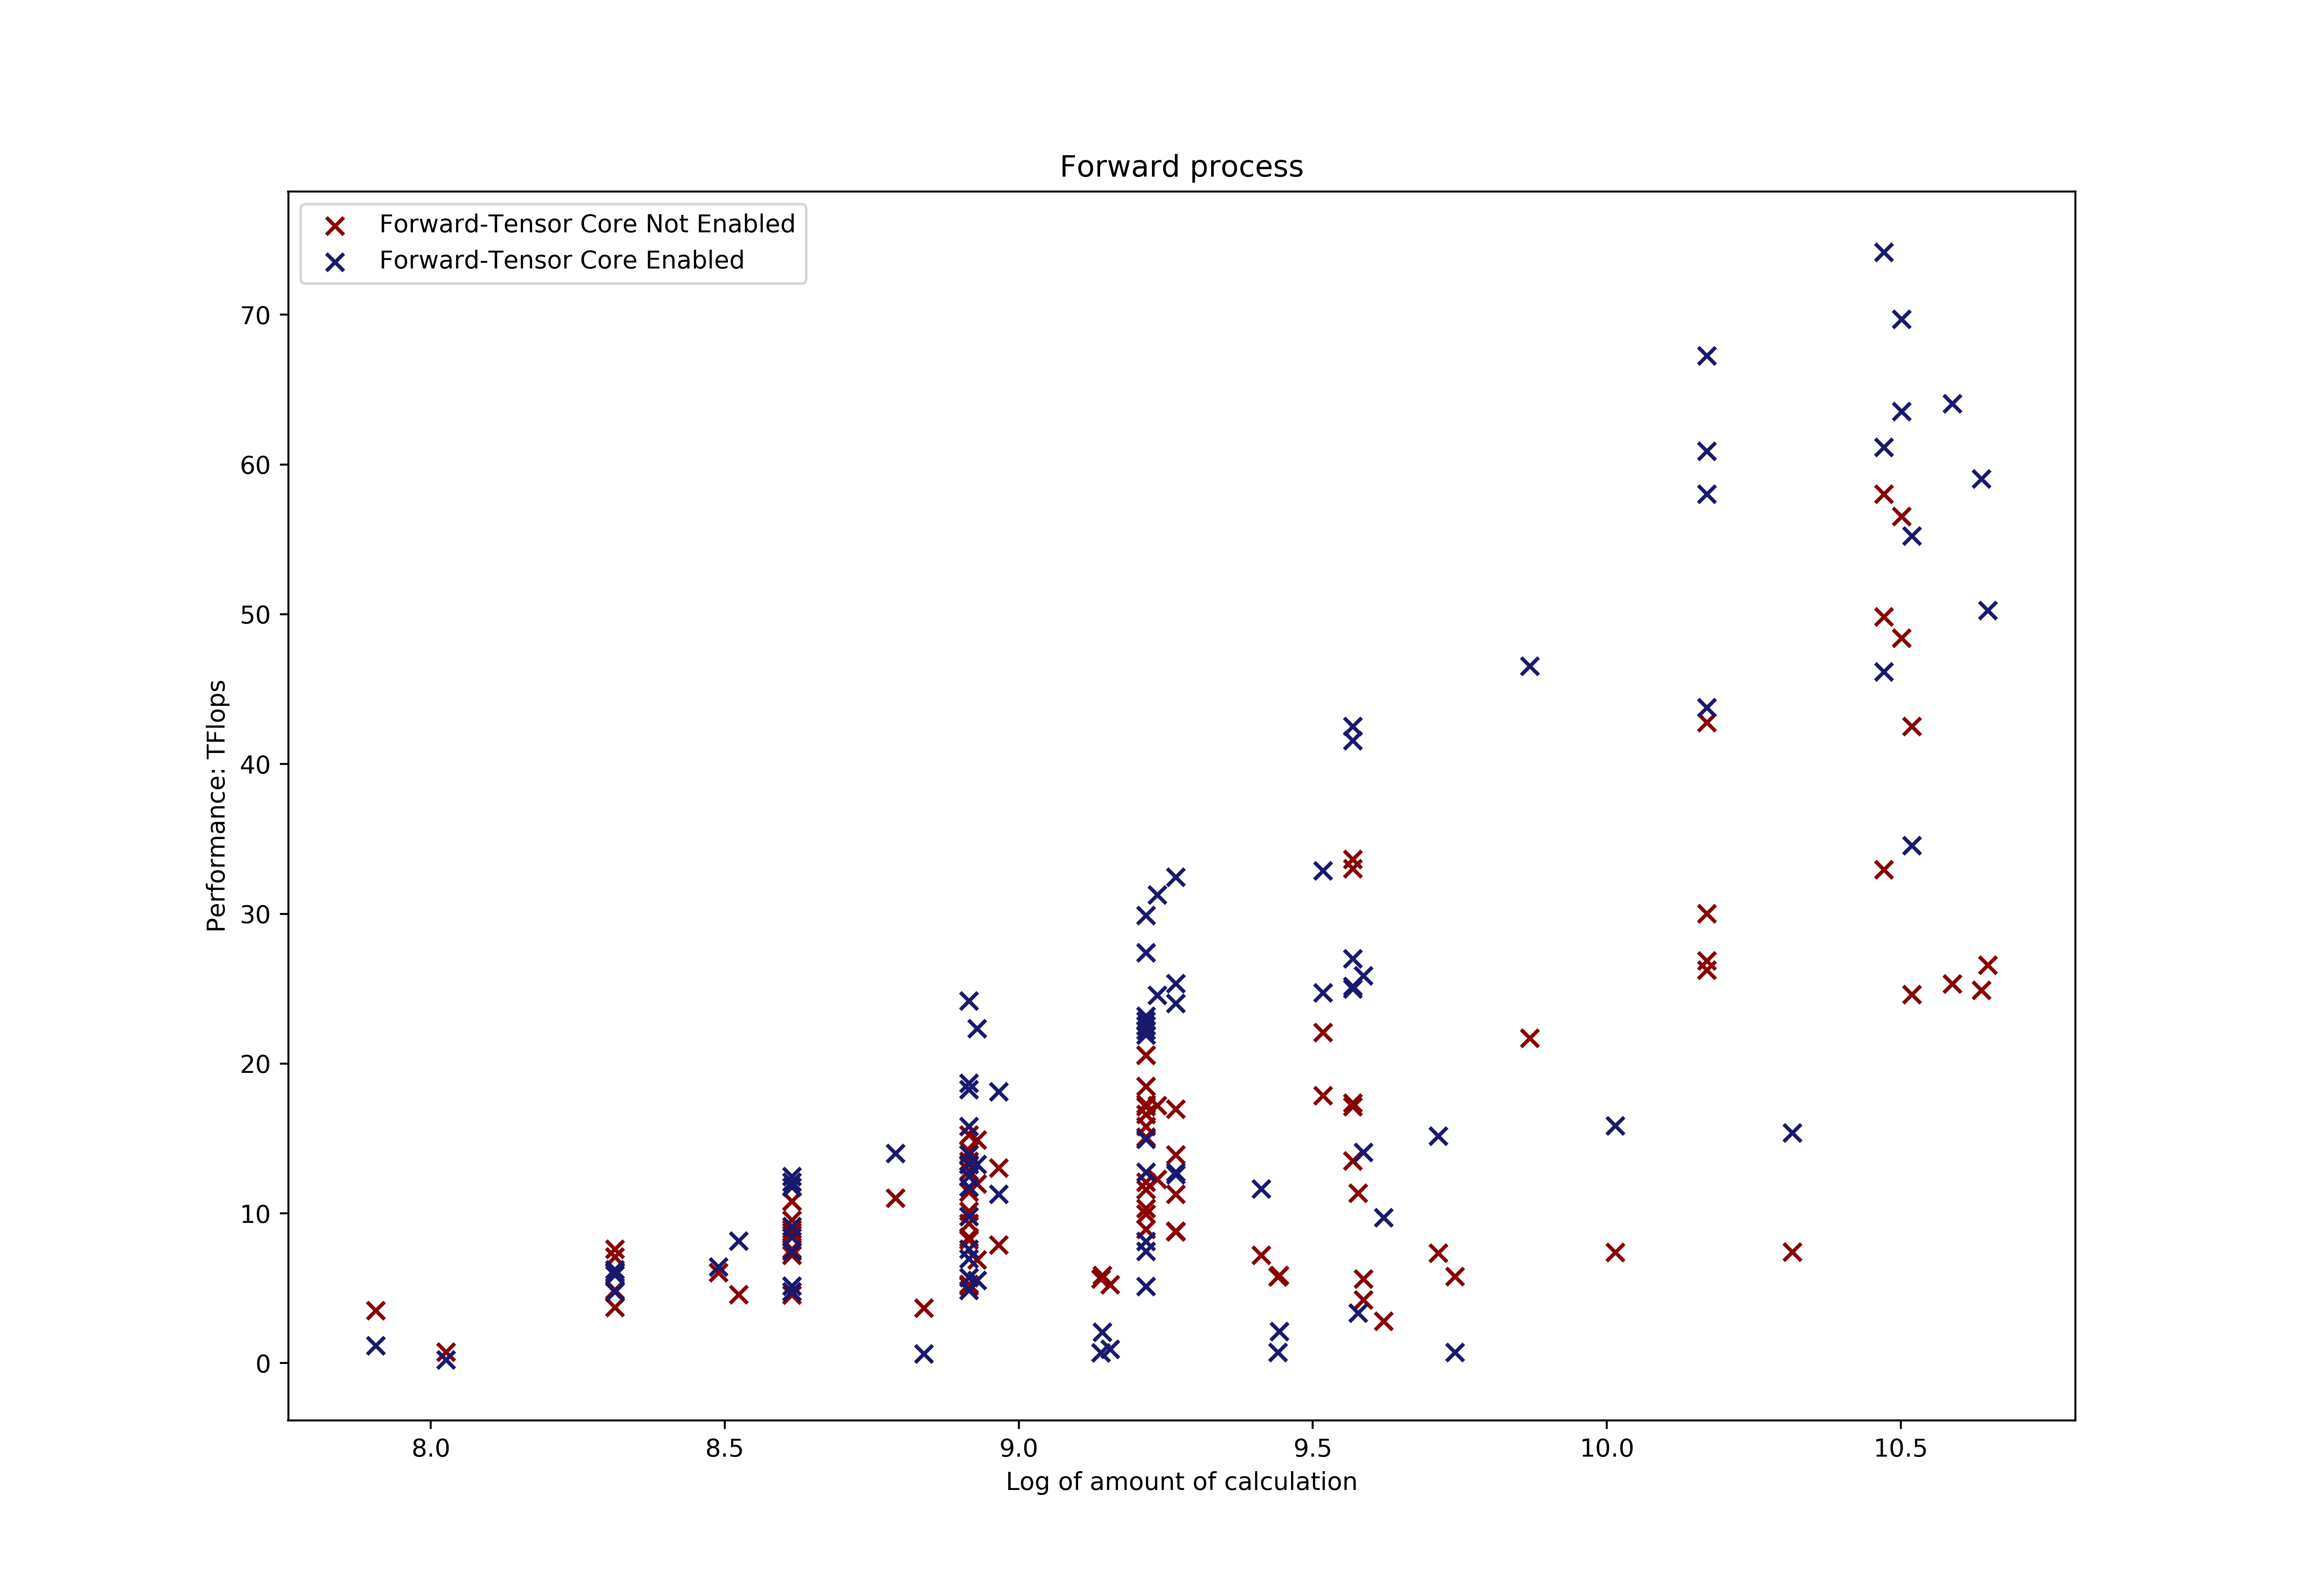
\includegraphics[width=4.5cm]{figures/CNN-HALF-FWD.jpg}
			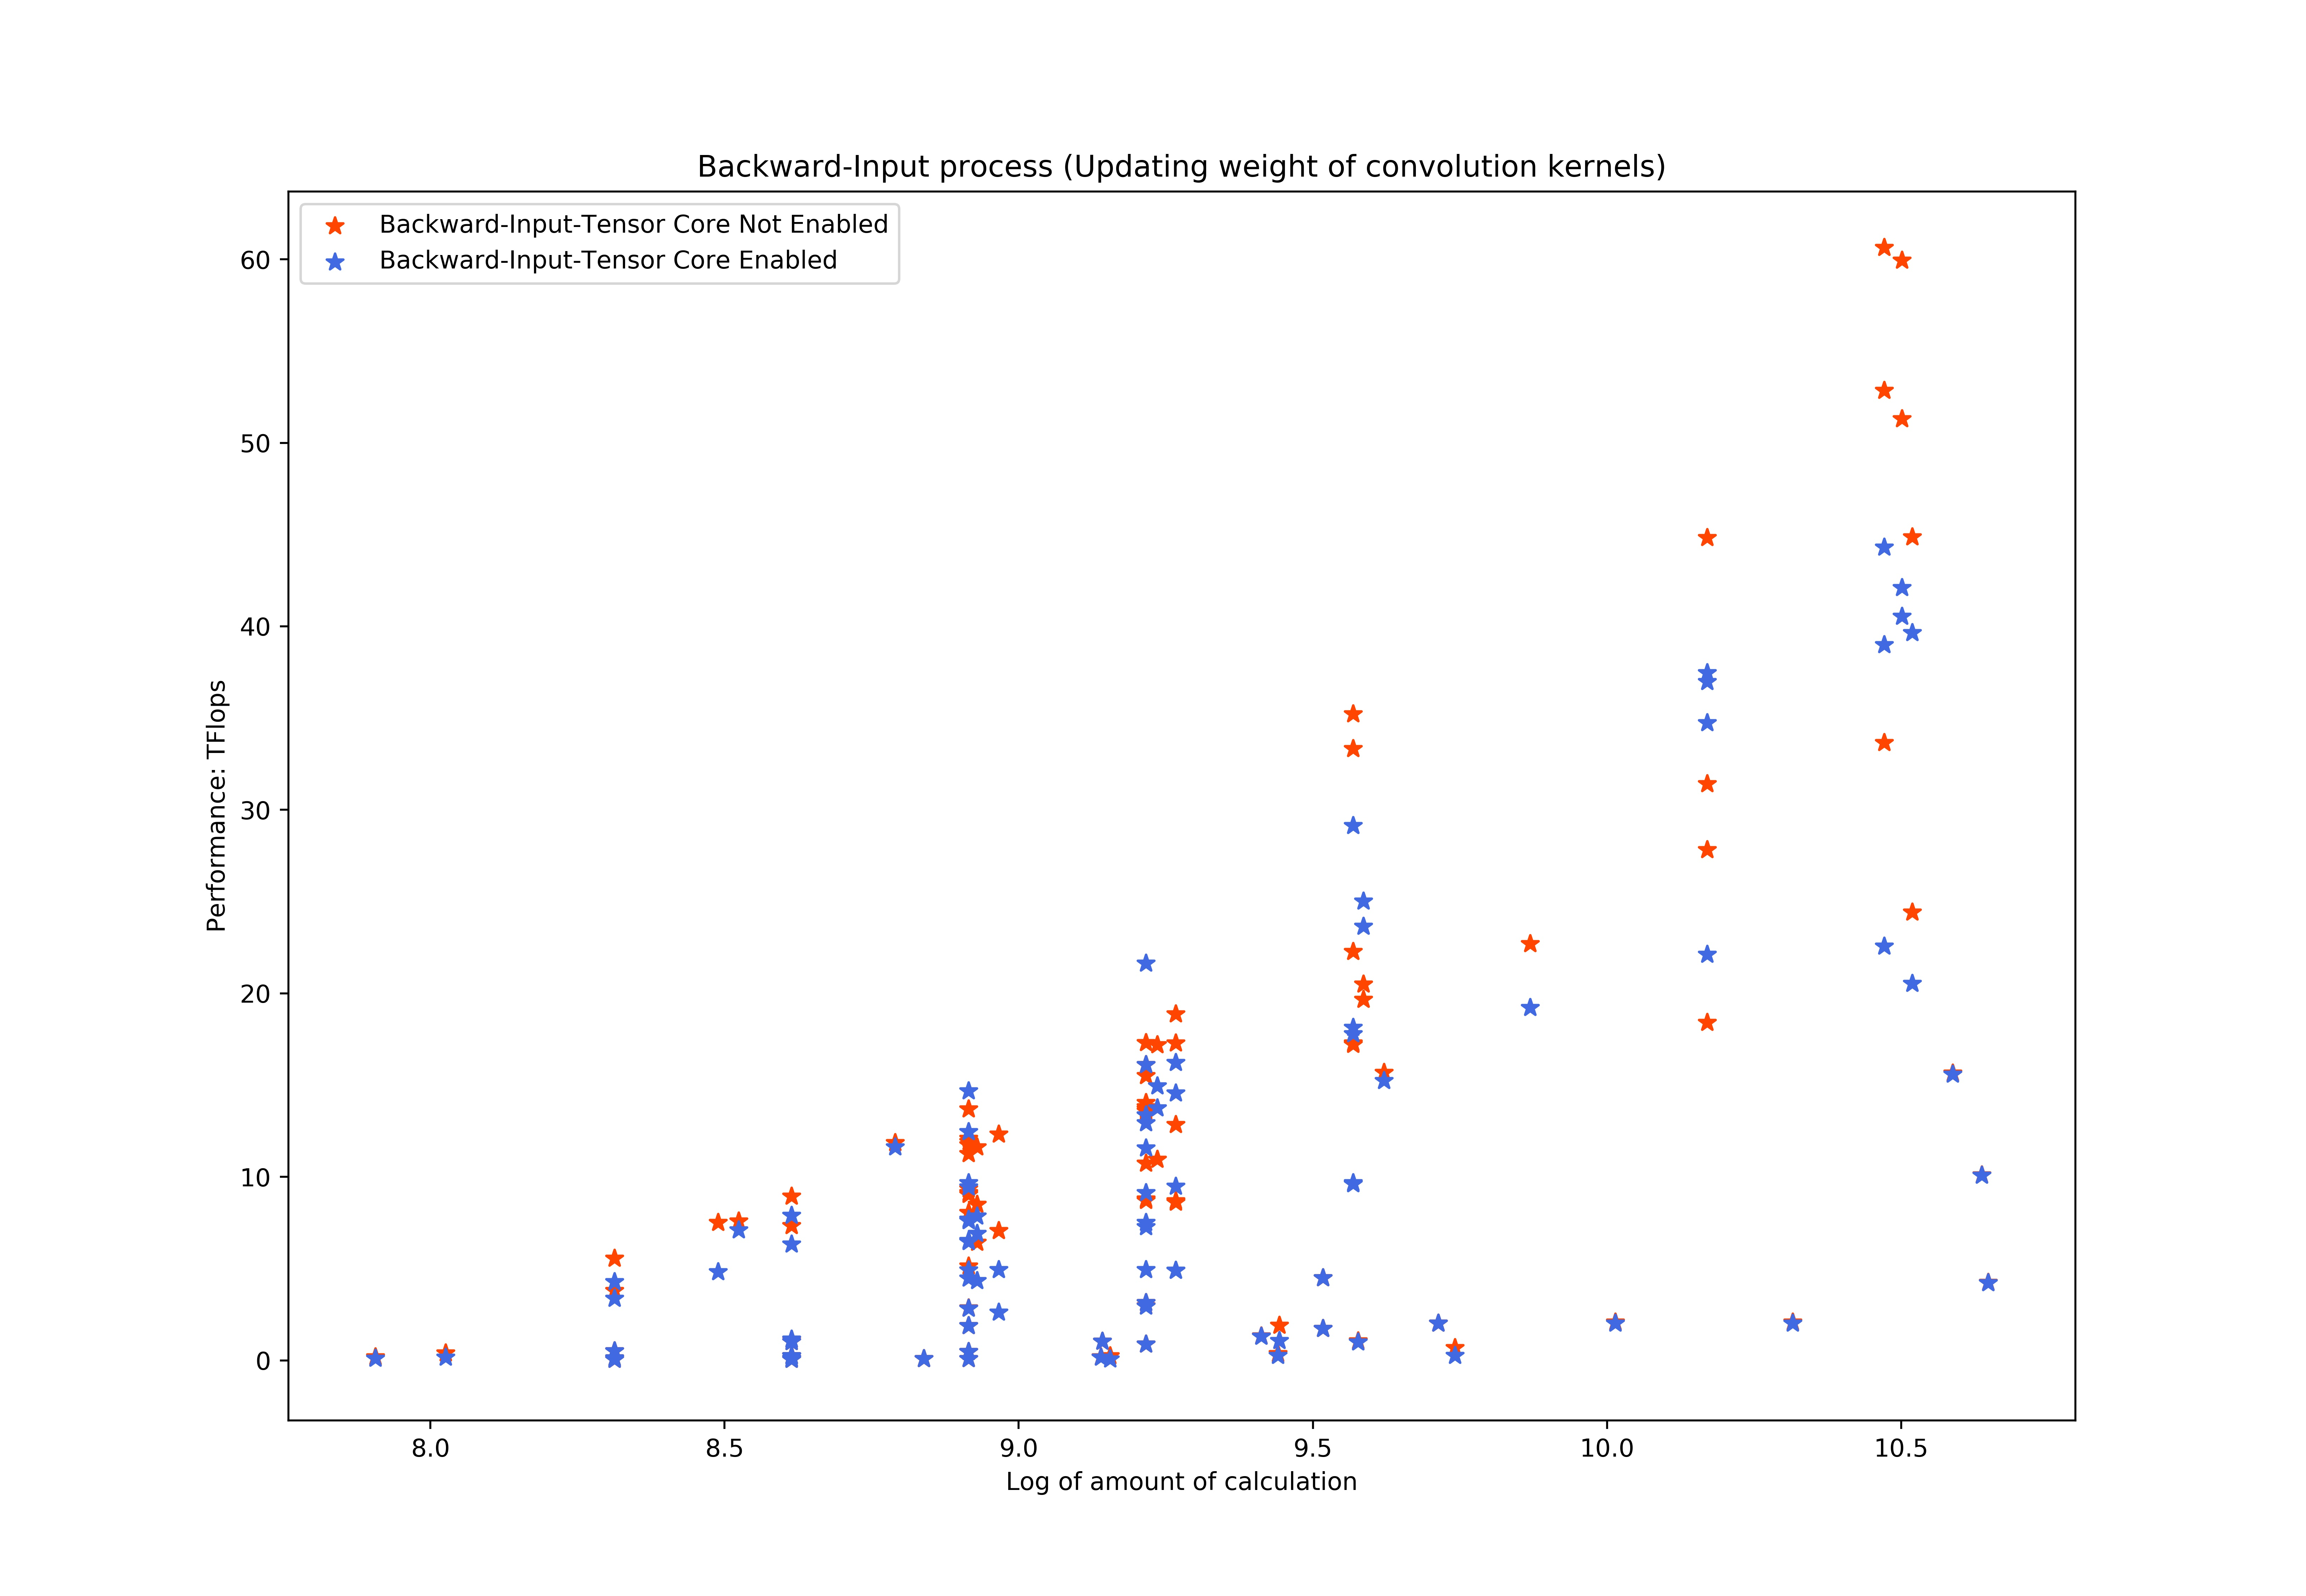
\includegraphics[width=4.5cm]{figures/CNN-HALF-BWD-FILTER.jpg}
			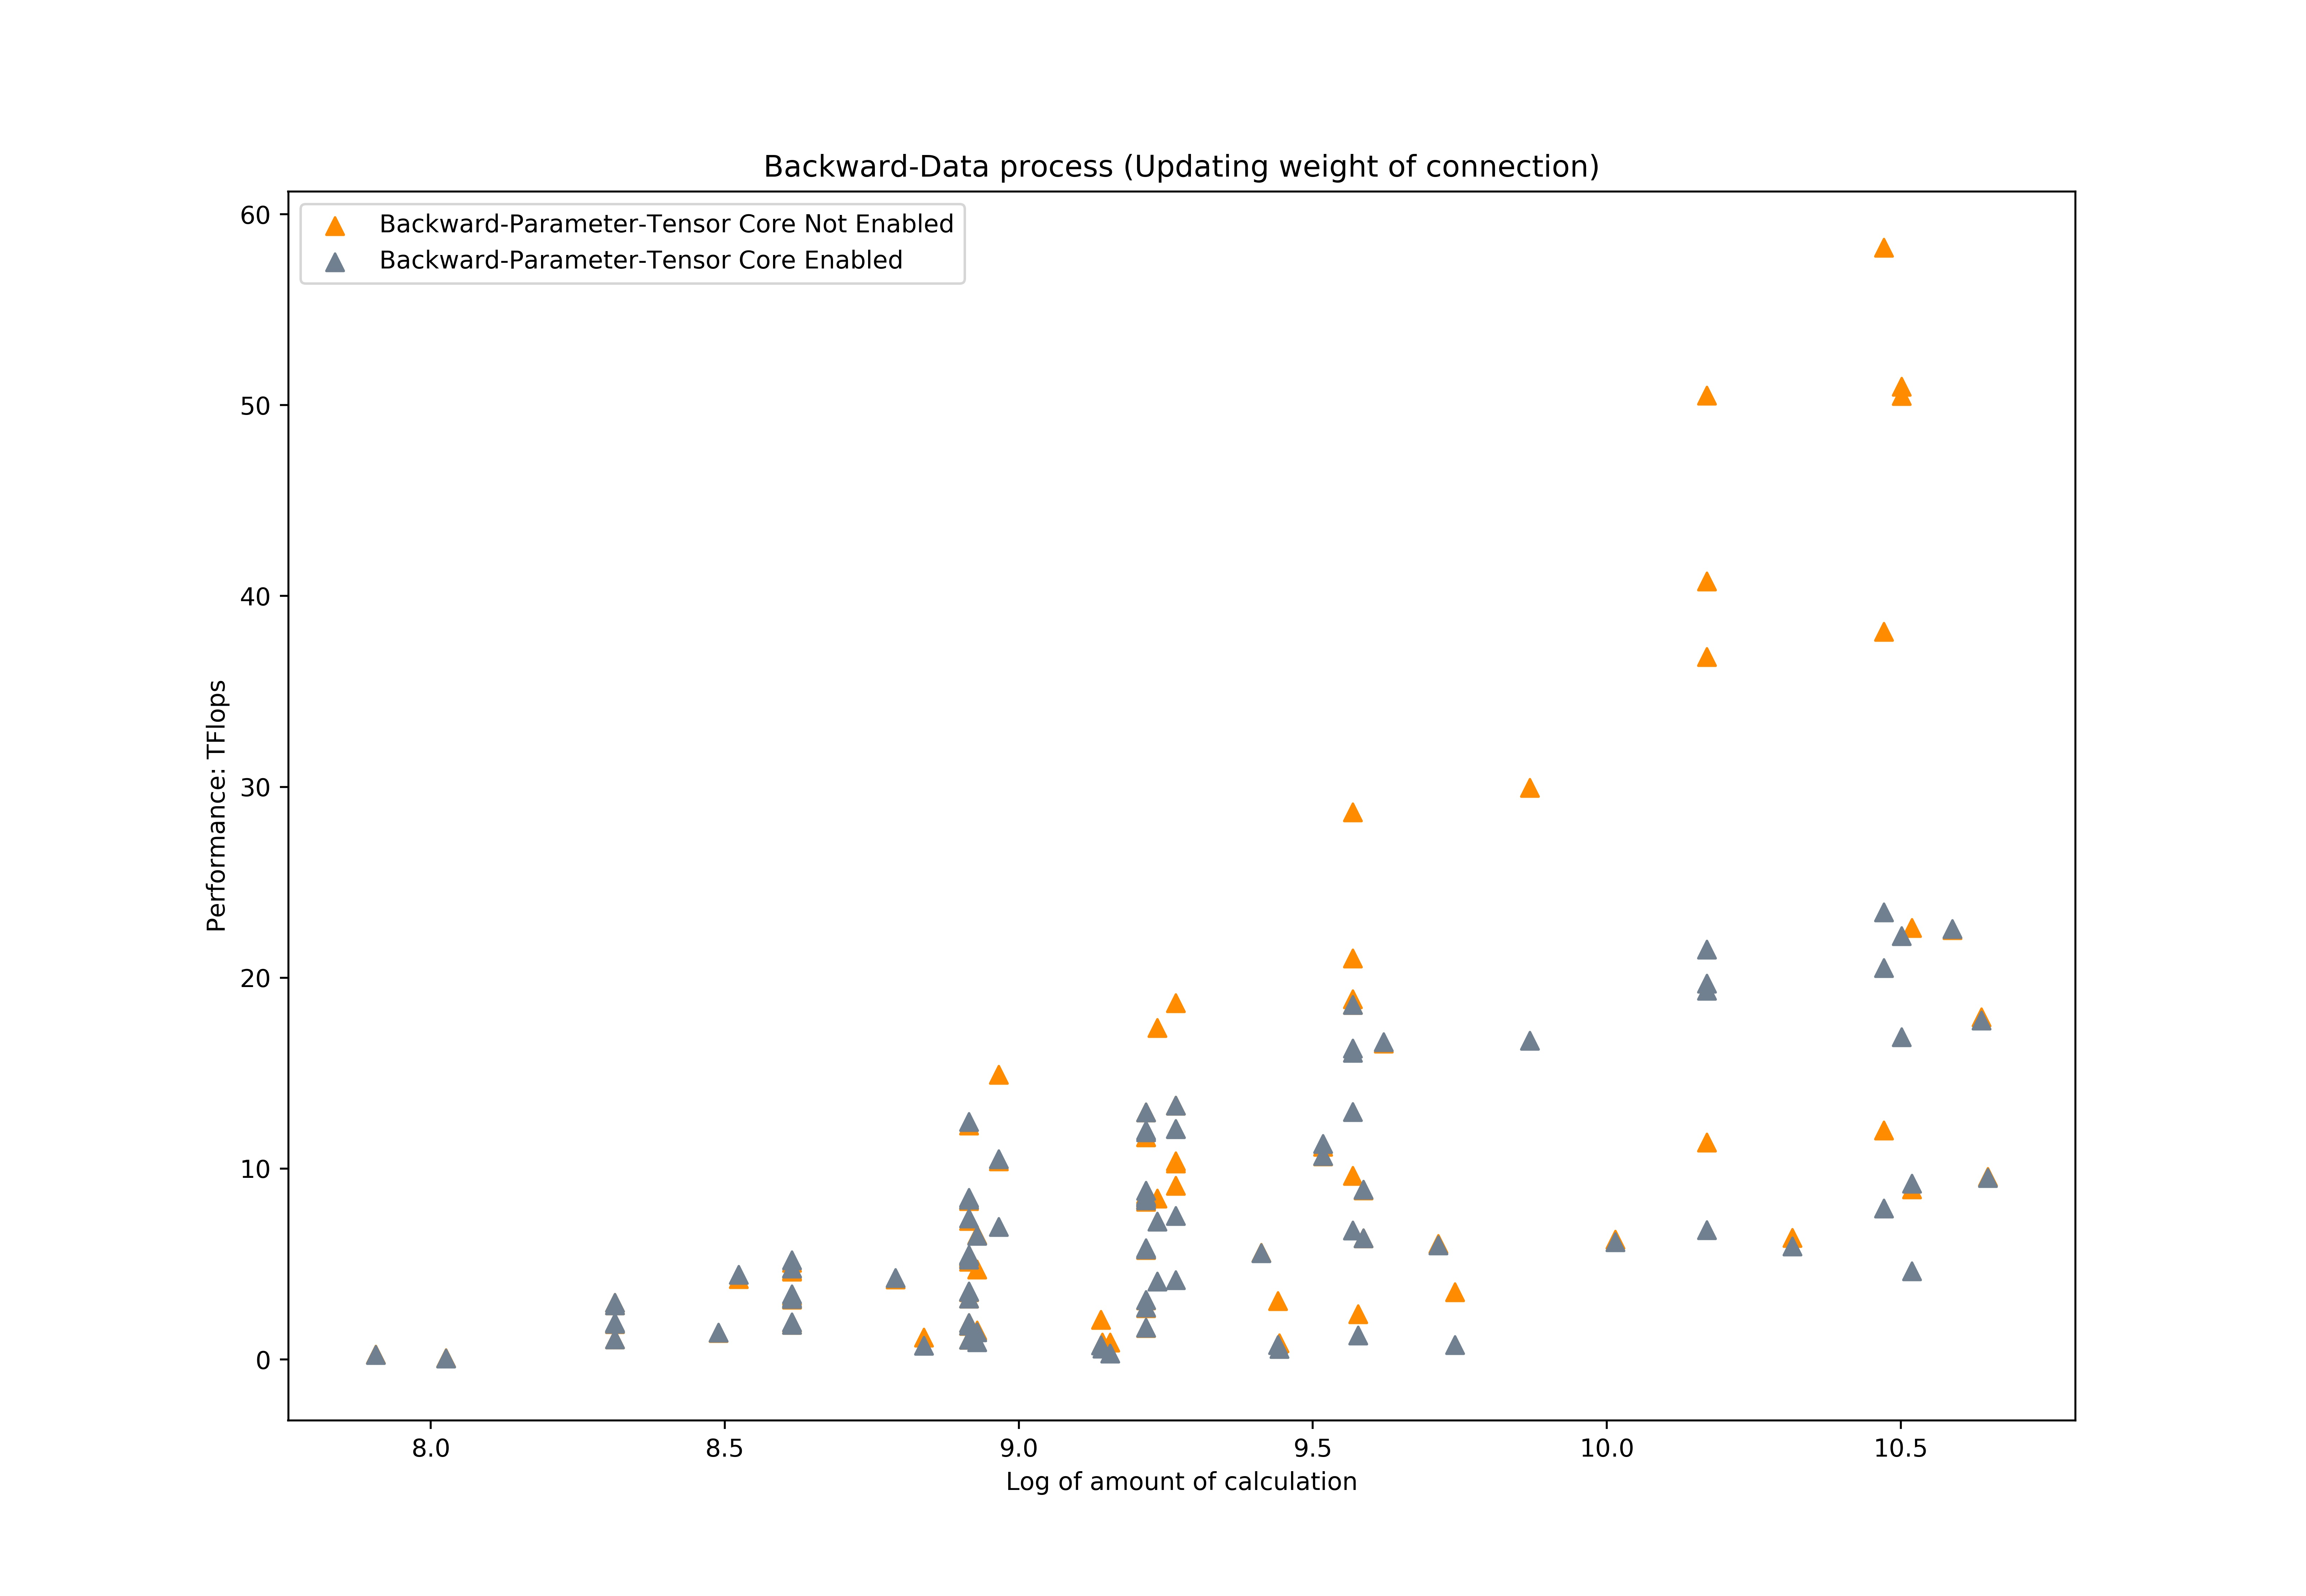
\includegraphics[width=4.5cm]{figures/CNN-HALF-BWD-DATA.jpg}
			% 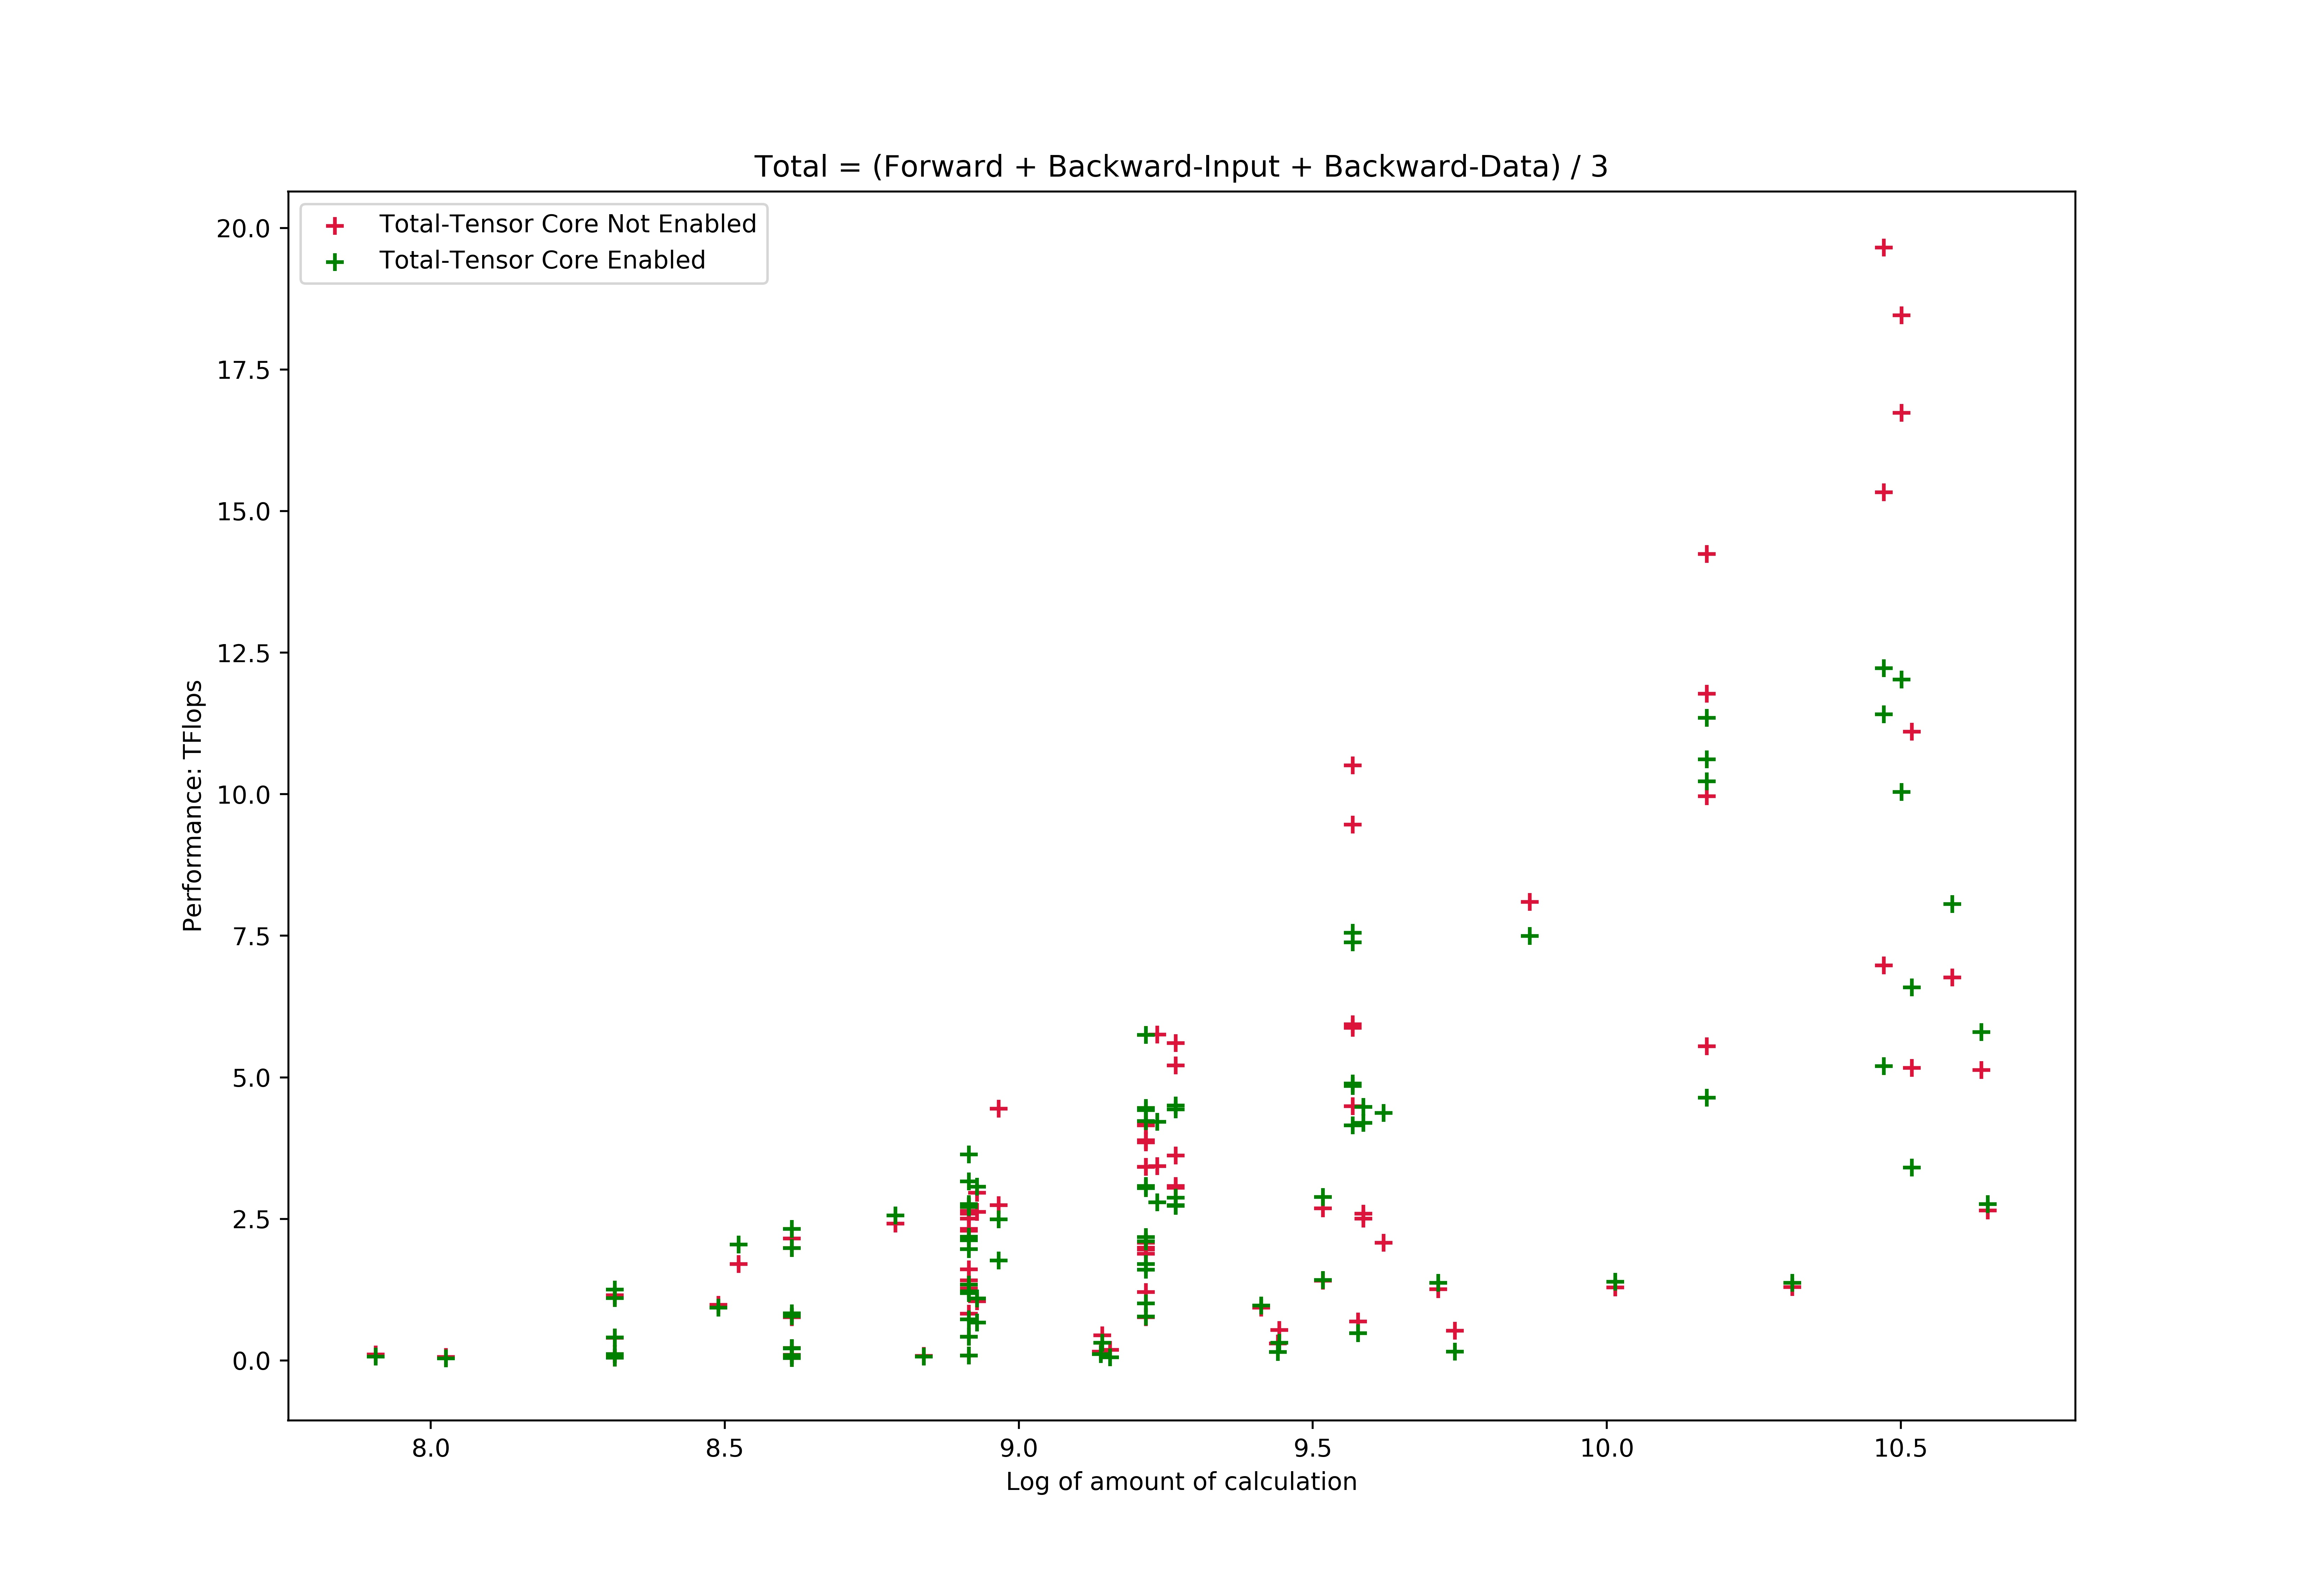
\includegraphics[width=4cm]{figures/CNN-HALF-TOTAL.jpg}\\
			\caption{不卷积神经网络不同过程的性能}\label{Fig.CONV3PART}
		\end{figure}
		除存在密集矩阵乘加、卷积运算的前向传播,其余部分开启张量核心后性能均有下降。由上节图像尺寸较小时使用基于纹理内存的直接计算方法取得较好的结果,尝试使用直接计算方法以及纹理内存进行优化。
	\end{frame}
	
	\begin{frame}
		\frametitle{CUDA C::卷积神经网络}
		\begin{figure}
			\centering
			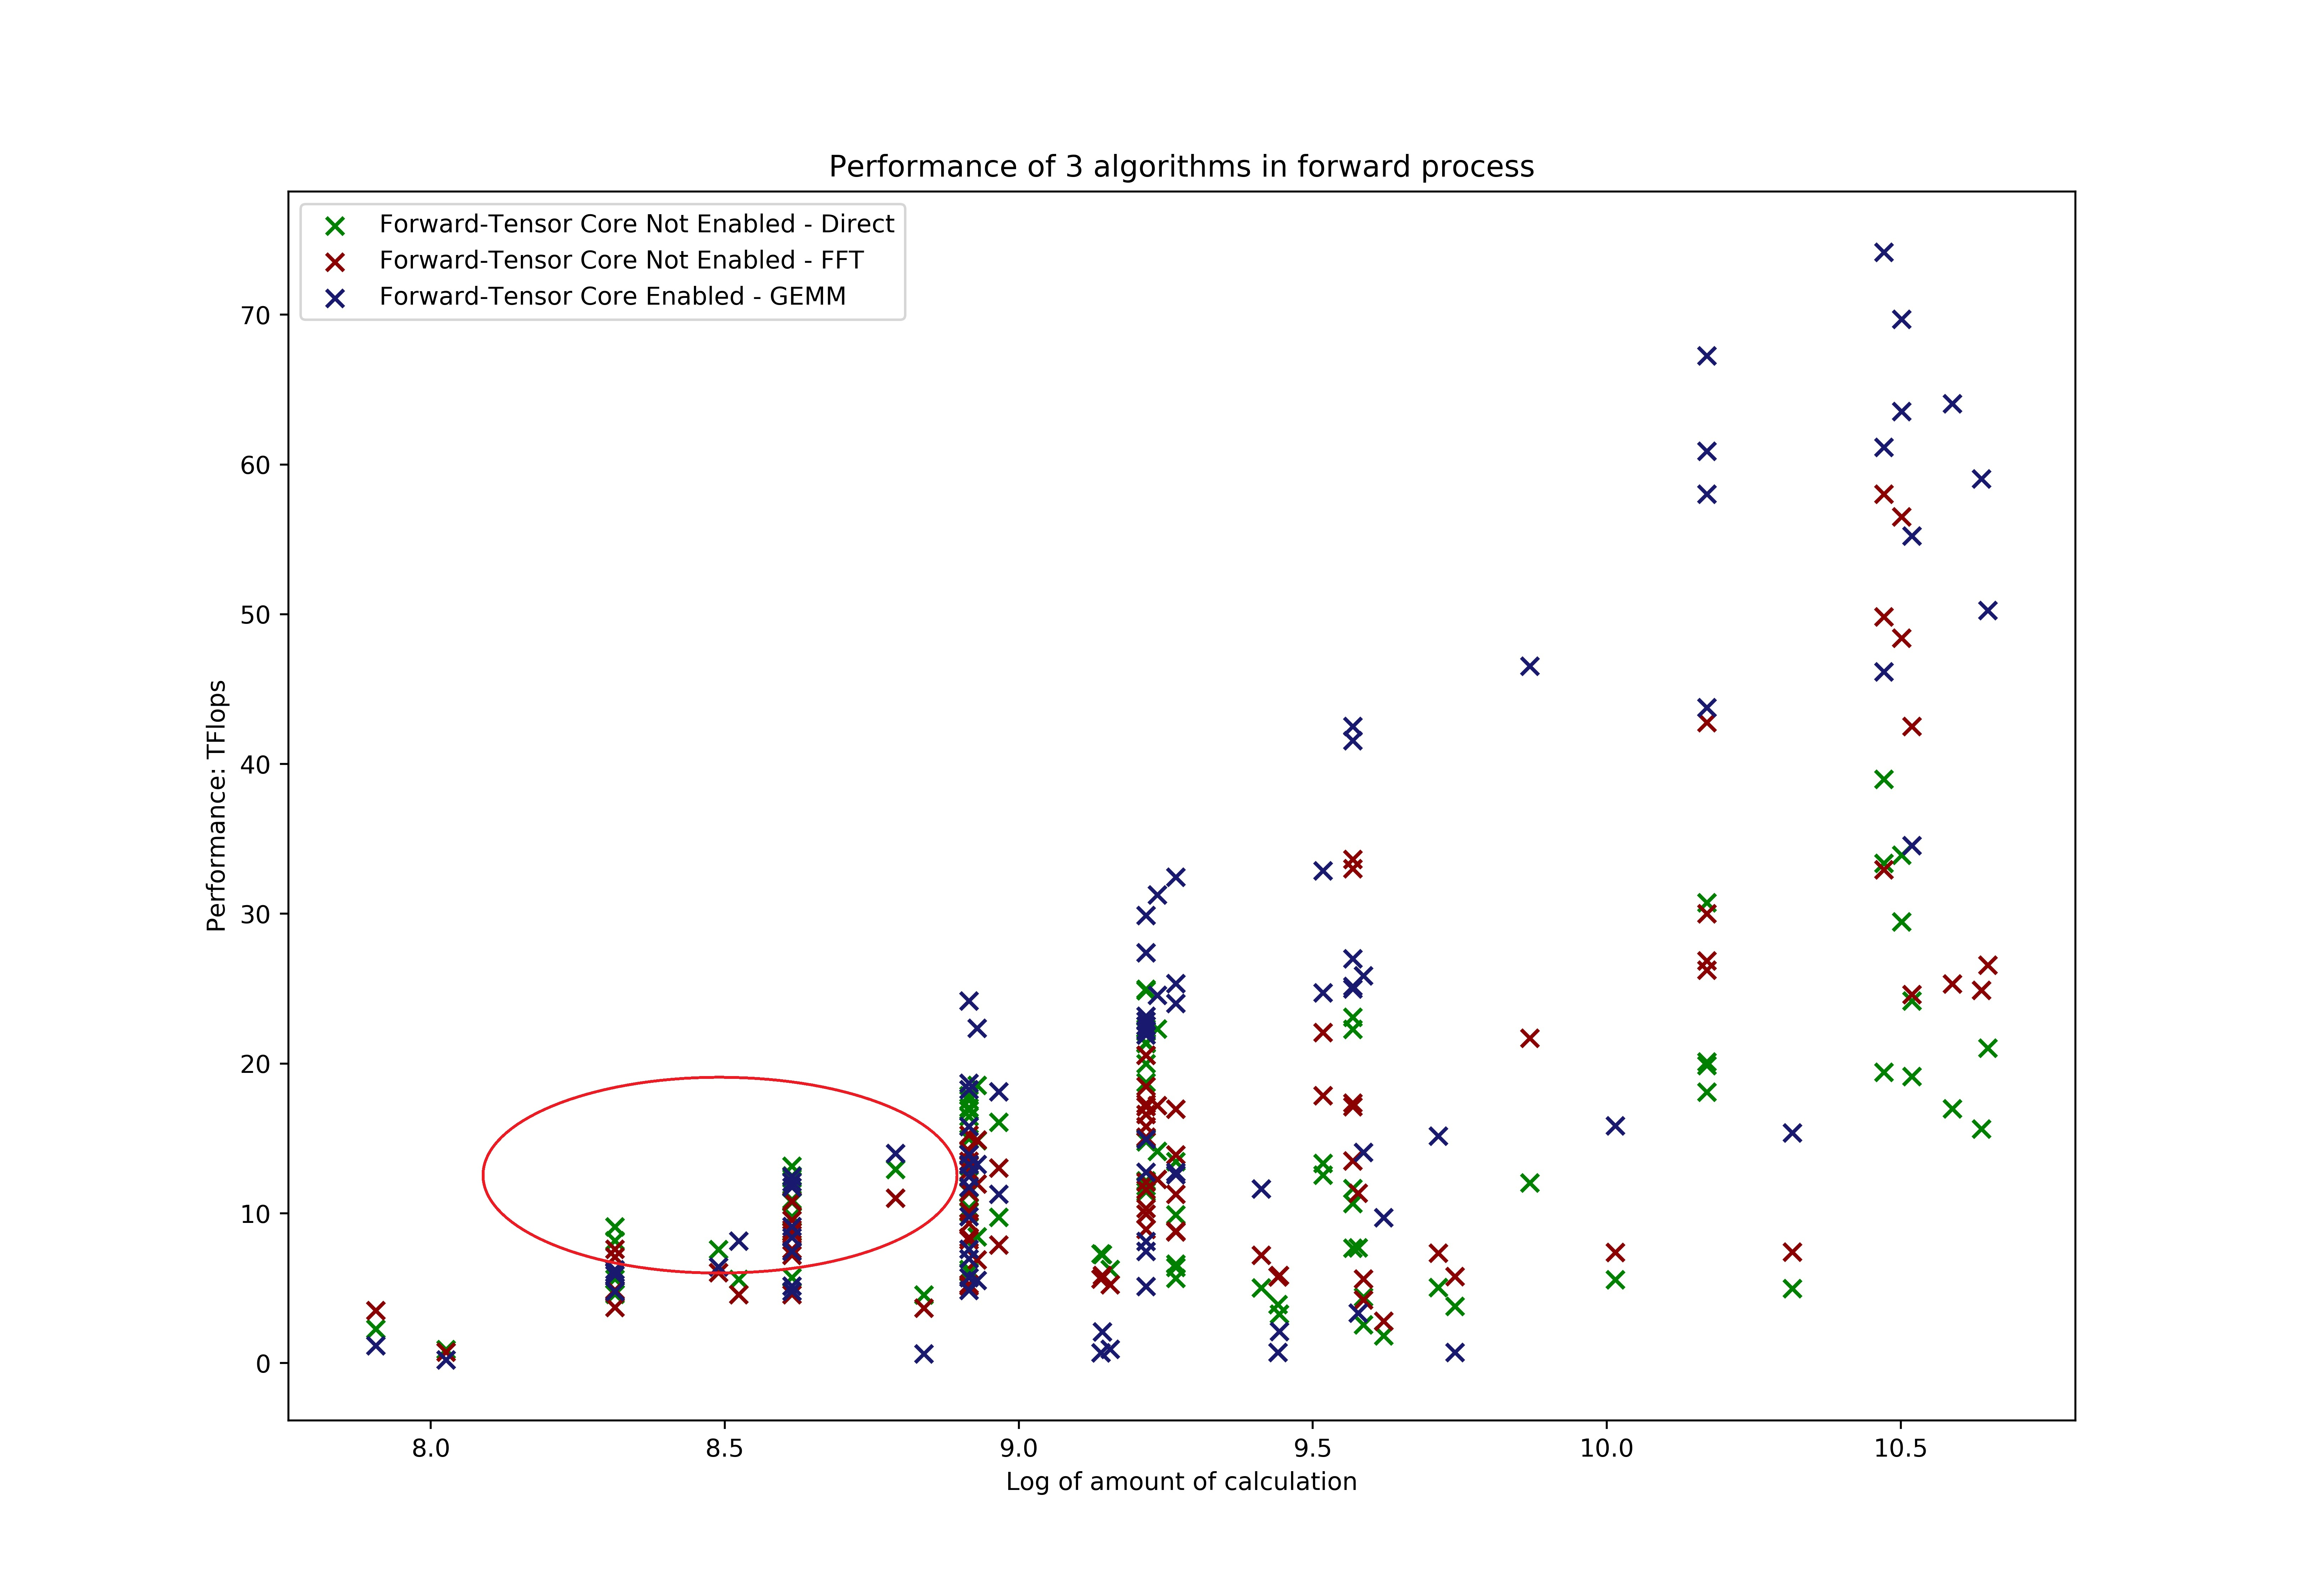
\includegraphics[width=5.5cm]{figures/CNN-HALF-3ALGOFWD.jpg}
			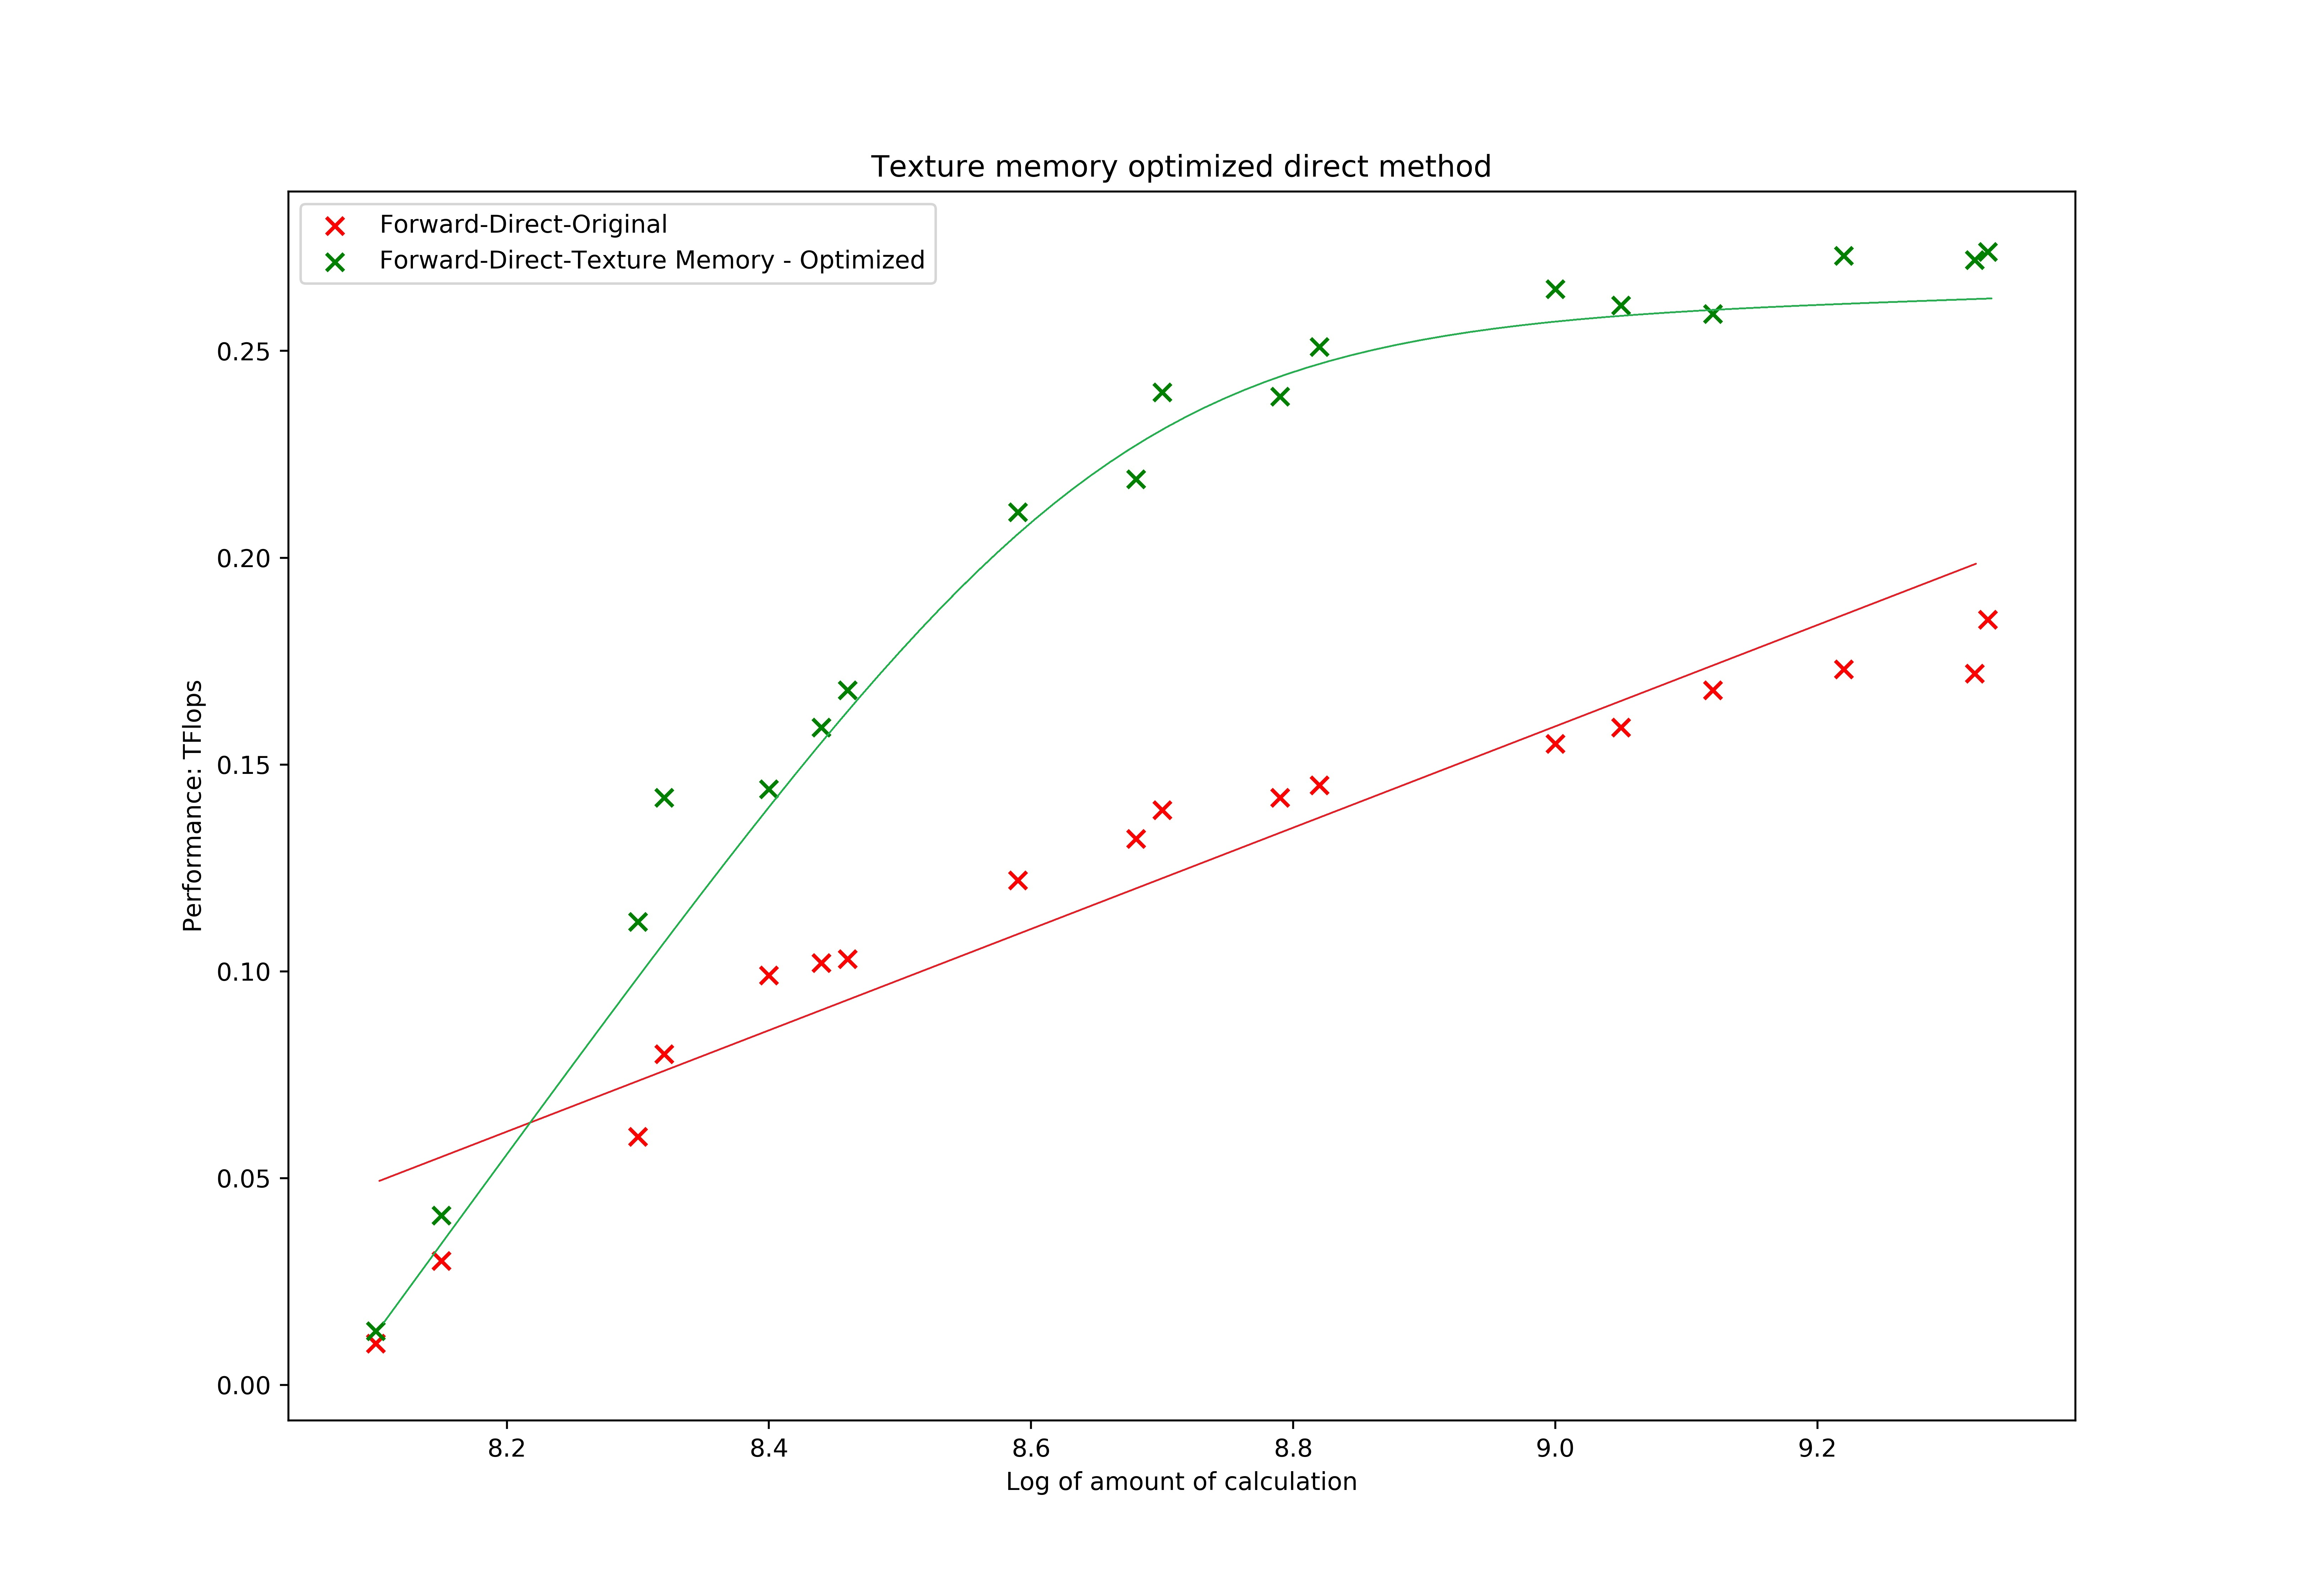
\includegraphics[width=5.5cm]{figures/CNN-HALF-TEXOPT.jpg}
			\caption{使用直接方法辅以纹理内存优化的卷积}\label{Fig.CONVTEX}
		\end{figure}
		可见在图像尺寸较小时该优化方式效果较好,随着图像尺寸增大,纹理内存的性能逐渐到达瓶颈。\\
		$ * $不使用纹理内存直接进行计算的理由为cuDNN封装底层计算,故采用这种间接比较的方式。
	\end{frame}
	
	\subsubsection{支持向量机(SMO-SVM)}
	\begin{frame}
		\frametitle{CUDA C::支持向量机} 
		最小序列优化支持向量机中涉及部分矩阵运算,且由于支持向量机特征向量的特点,使用稀疏矩阵进行优化会有较好的效果,本文采用了如下方法进行支持向量机中的矩阵运算。
		\begin{table}
			\centering
			\caption{SMO-SVM中的矩阵计算方式}
			\begin{tabular}{cc}
				\toprule
				矩阵计算方法 & 描述	\\
				\midrule
				GEMM Legacy & 基于老架构、老SDK的GEMM实现方式\\
				GEMM & 基于新架构、新SDK的不使用张量核心的实现方式\\
				GEMM Tensor Core& 基于新架构、新SDK的使用张量核心的实现方式\\
				cuSPARSE & 基于稀疏矩阵库的实现方式\\
				\bottomrule
			\end{tabular} \label{table-SMOSVM} 
		\end{table}
	\end{frame}
	\begin{frame}
		\frametitle{CUDA C::支持向量机}
		\begin{figure}
			\centering
			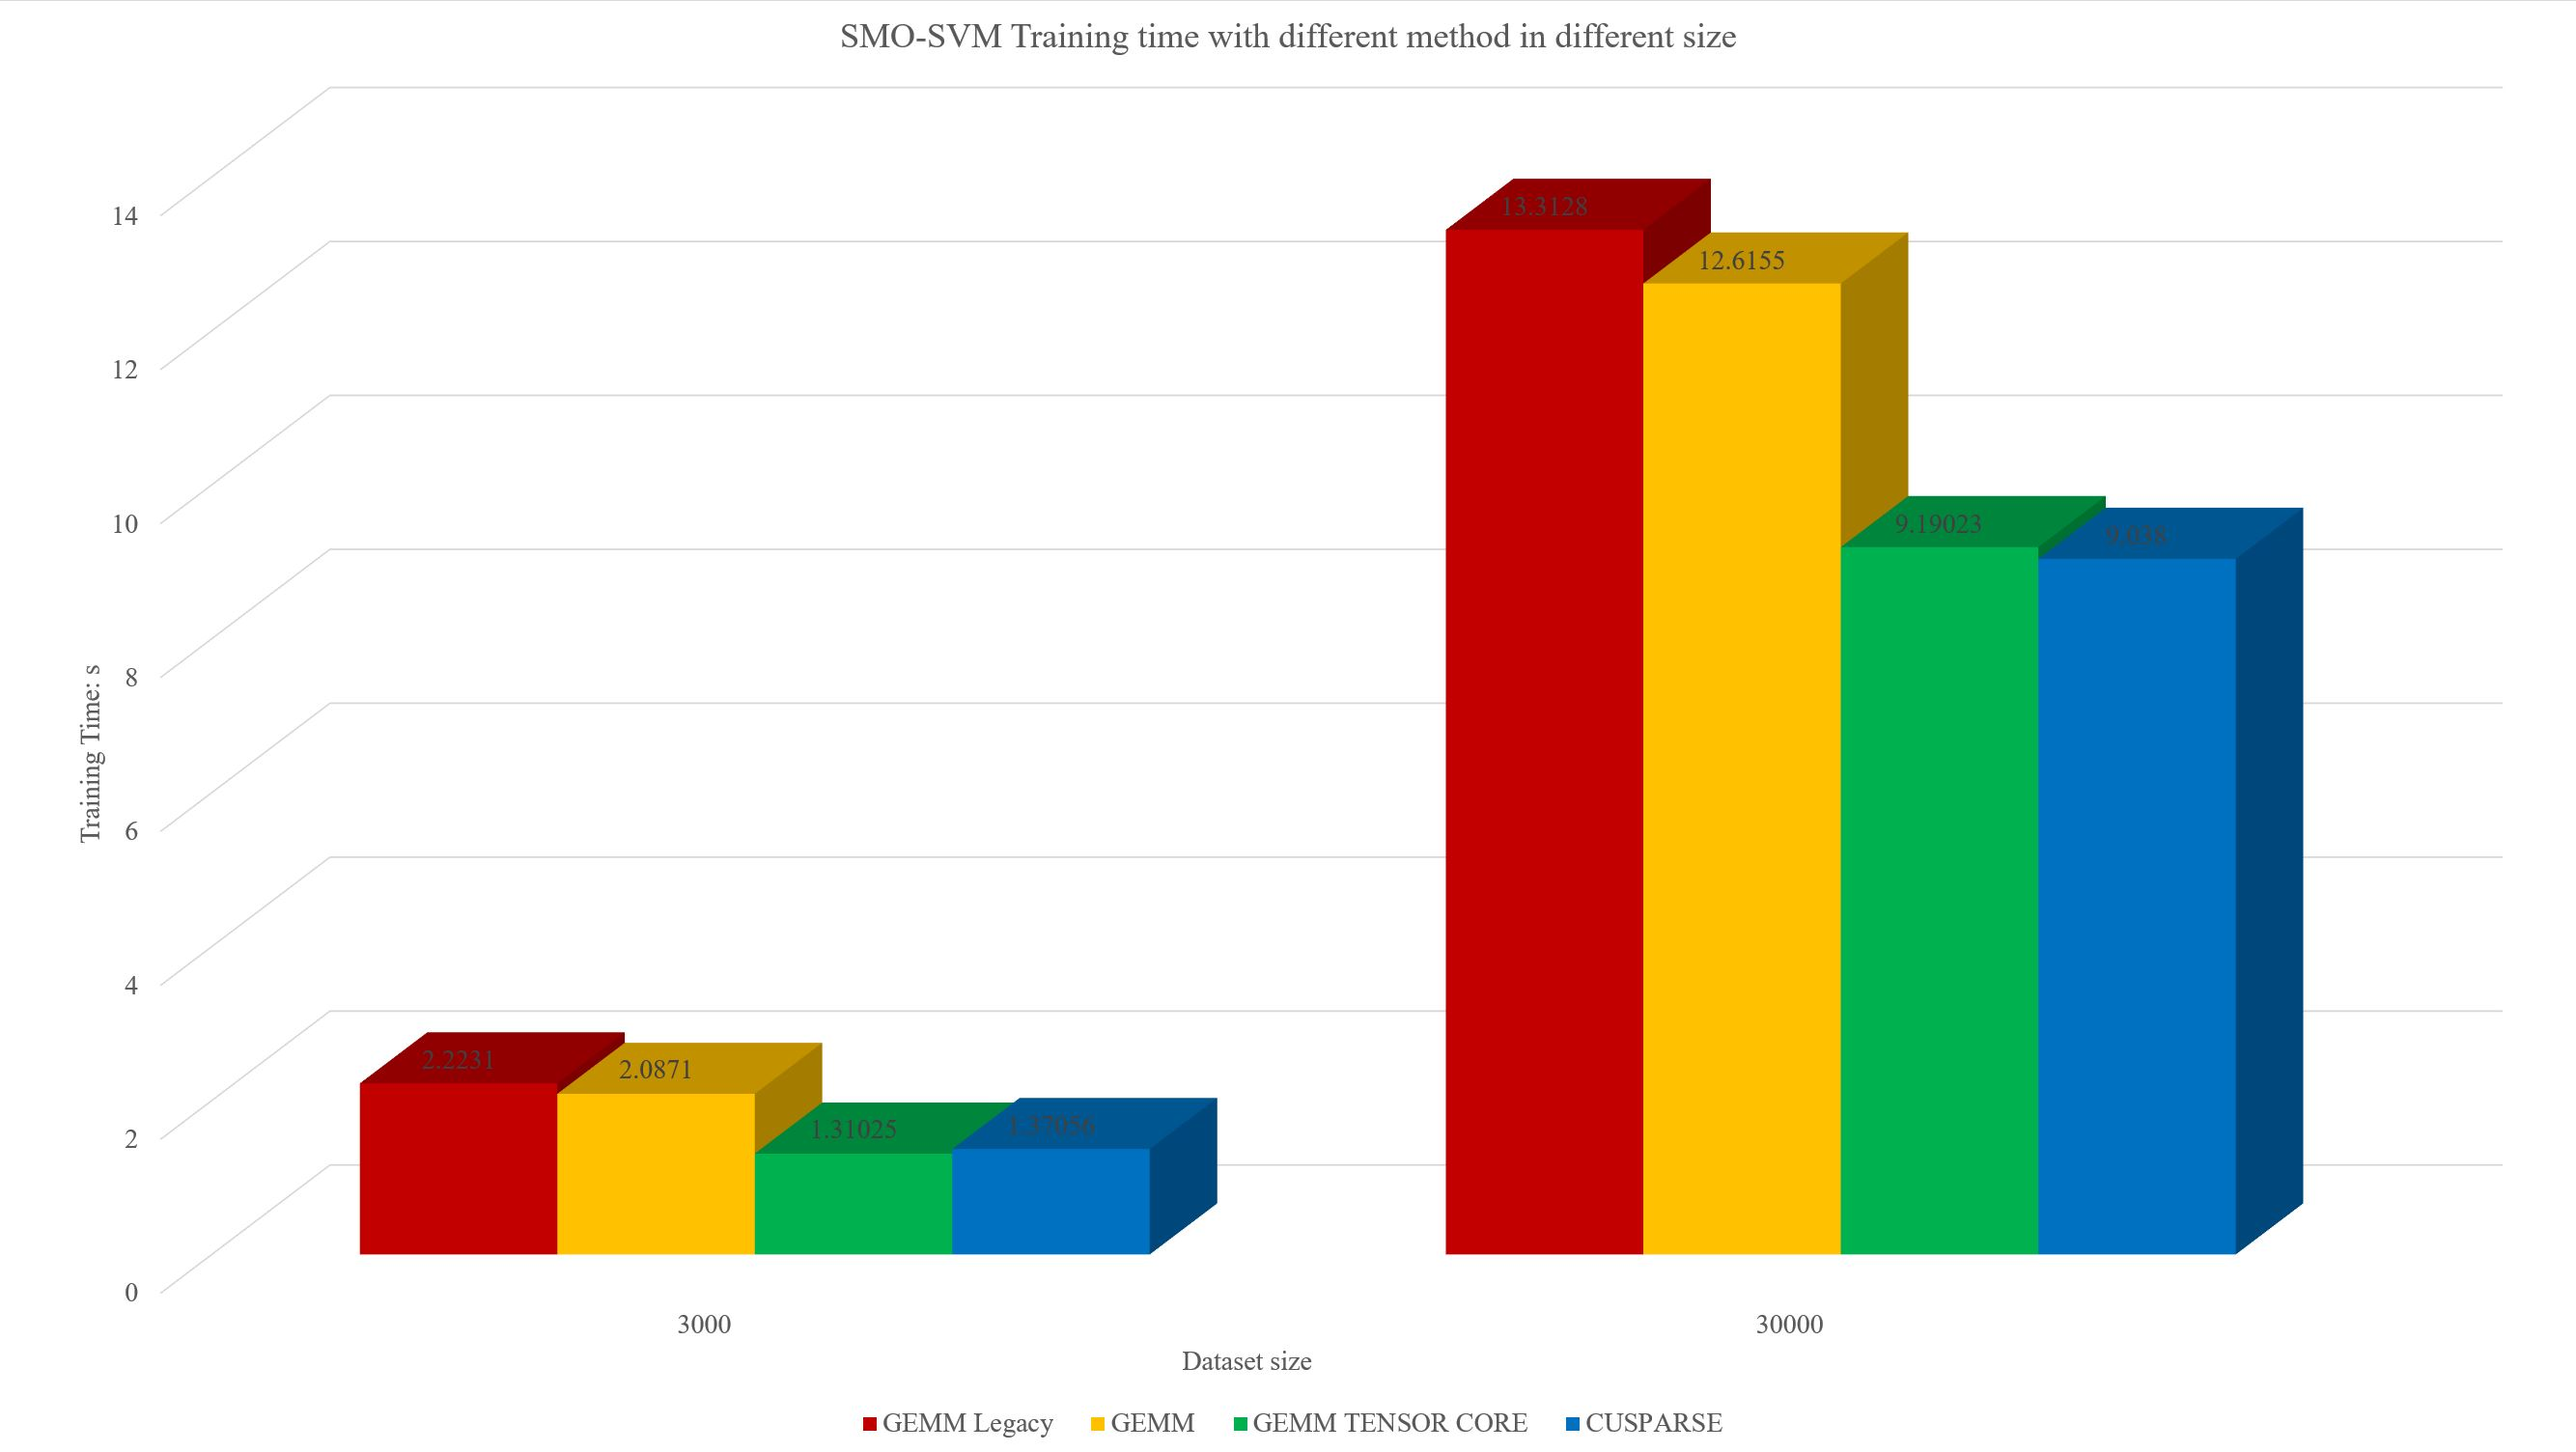
\includegraphics[width=7cm]{figures/SMOSVMRES.jpg}
			\caption{SMO-SVM训练时间}\label{Fig.SMOSVM}
		\end{figure}
		在数据条目较多、维度较高时由于特征较为稀疏,CSR压缩方式能取得较大压缩比,使用CUDA中cuSPARSE中为稀疏矩阵优化的API能取得较高的性能,而条目较小时CSR压缩方式压缩比较小,此时使用张量核心进行GEMM运算能取得较好的效果。\textbf{那么能否进一步对GEMM指令wmma进行稀疏矩阵优化呢}
	\end{frame}

	
	\subsection{TensorRT}
	\begin{frame}
		\frametitle{TensorRT与Jetson优化推理}
		之前的章节阐述了机器学习应用训练阶段新架构GPU的性能提升的研究与评估。而神经网络广泛用于嵌入式设备,对推理延迟要求较高,故本节考察不同网络结构采用TensorRT进行优化,采用Jetson TX2作为目标硬件进行评估。网络结构及特征如下表所示。
		\begin{table}
			\centering
			\caption{网络推理实验中使用的网络及特点}
			\begin{tabular}{cc}
				\toprule
				网络结构	&	描述\\
				\midrule
				Inception\_v1 & 网络深度、宽度较大,总体计算量较大\\
				ResNet\_v2 & 引入残差解决梯度、过拟合问题,网络可以更深\\
				Inveption\_v3 & 引入批归一化,使用$ 1\times n, n\times 1 $代替$ n\times n $卷积,卷积形状不同\\
				Inveption\_v4 & 使用残差优化的Inception\_v3\\
				Inveption\_resnet\_v2 & 结合Invenption与ResNet而生,与Inception\_v4较相似\\
				\textbf{mobileNet\_v1} & \textbf{压缩网络规模,将标准卷积分解为深度卷积和逐点卷积}\\
				\textbf{vgg\_16} &  \textbf{结构简化,但参数数量异常巨大,达1.38亿}\\
				\bottomrule
			\end{tabular} 
		\end{table}
		
	\end{frame}
	\begin{frame}
		\frametitle{TensorRT与Jetson优化推理}
		\begin{figure}
			\centering
			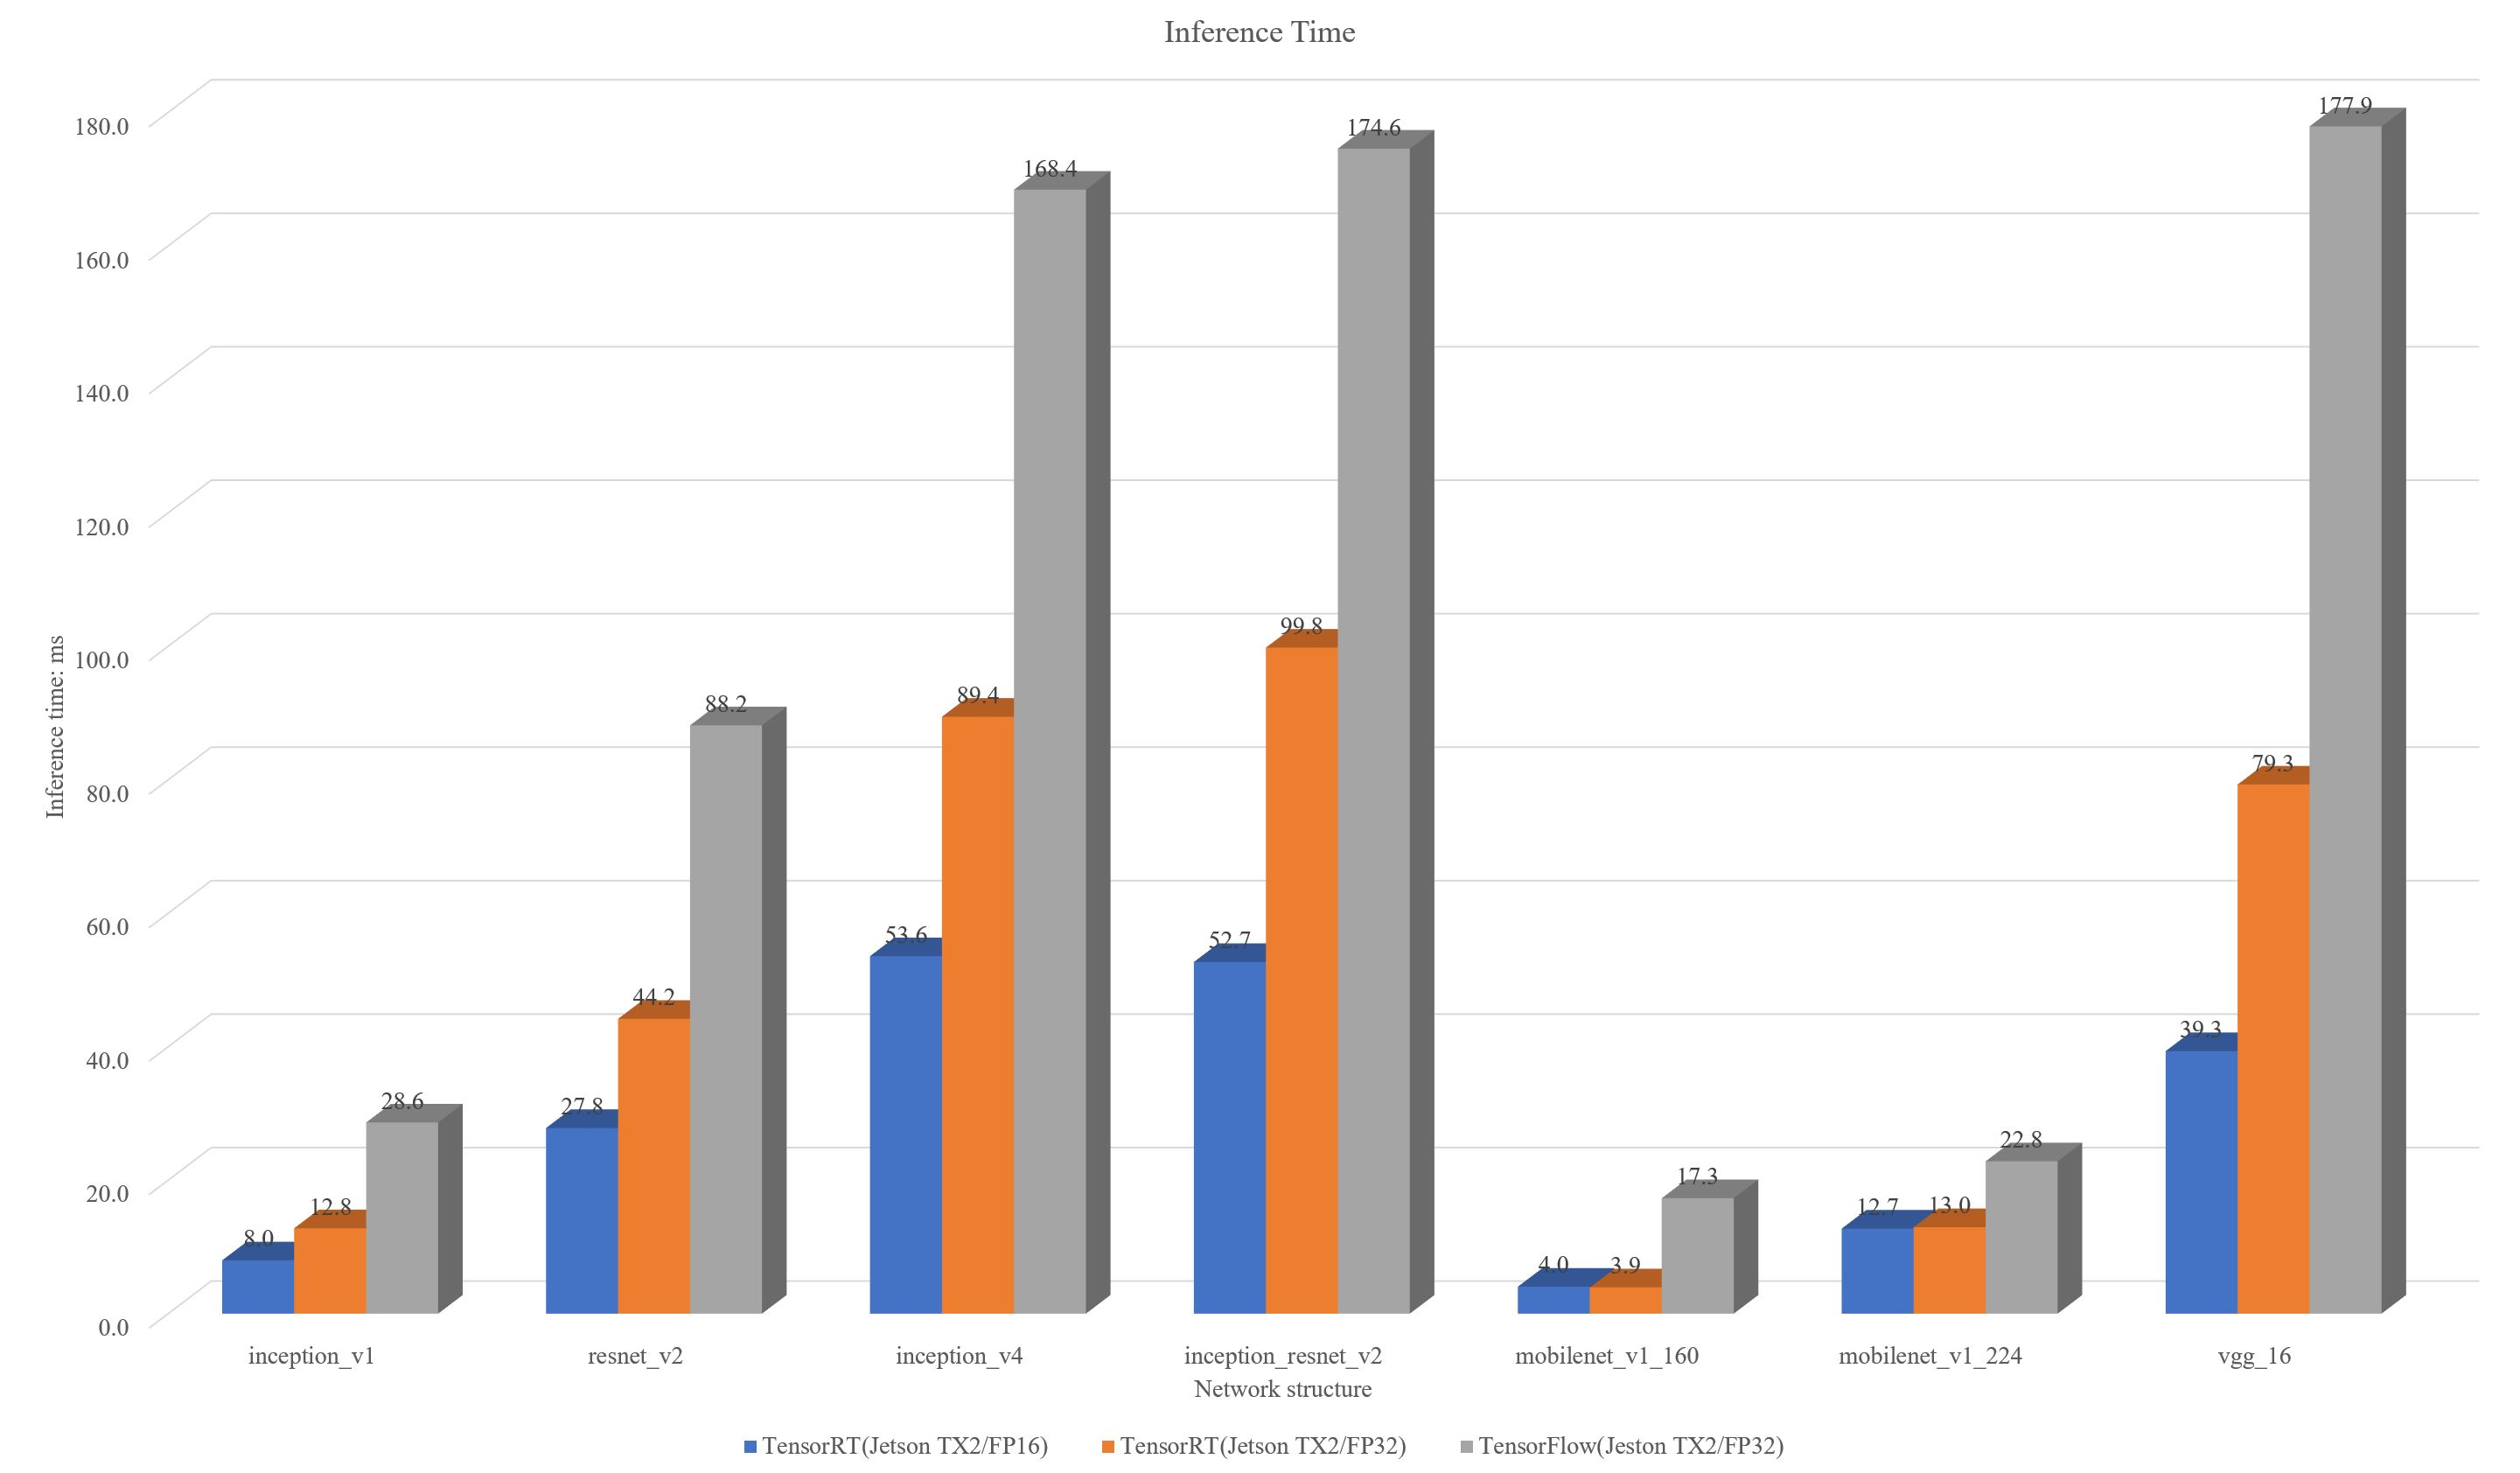
\includegraphics[width=5.5cm]{figures/TENSORRTRES.jpg}
			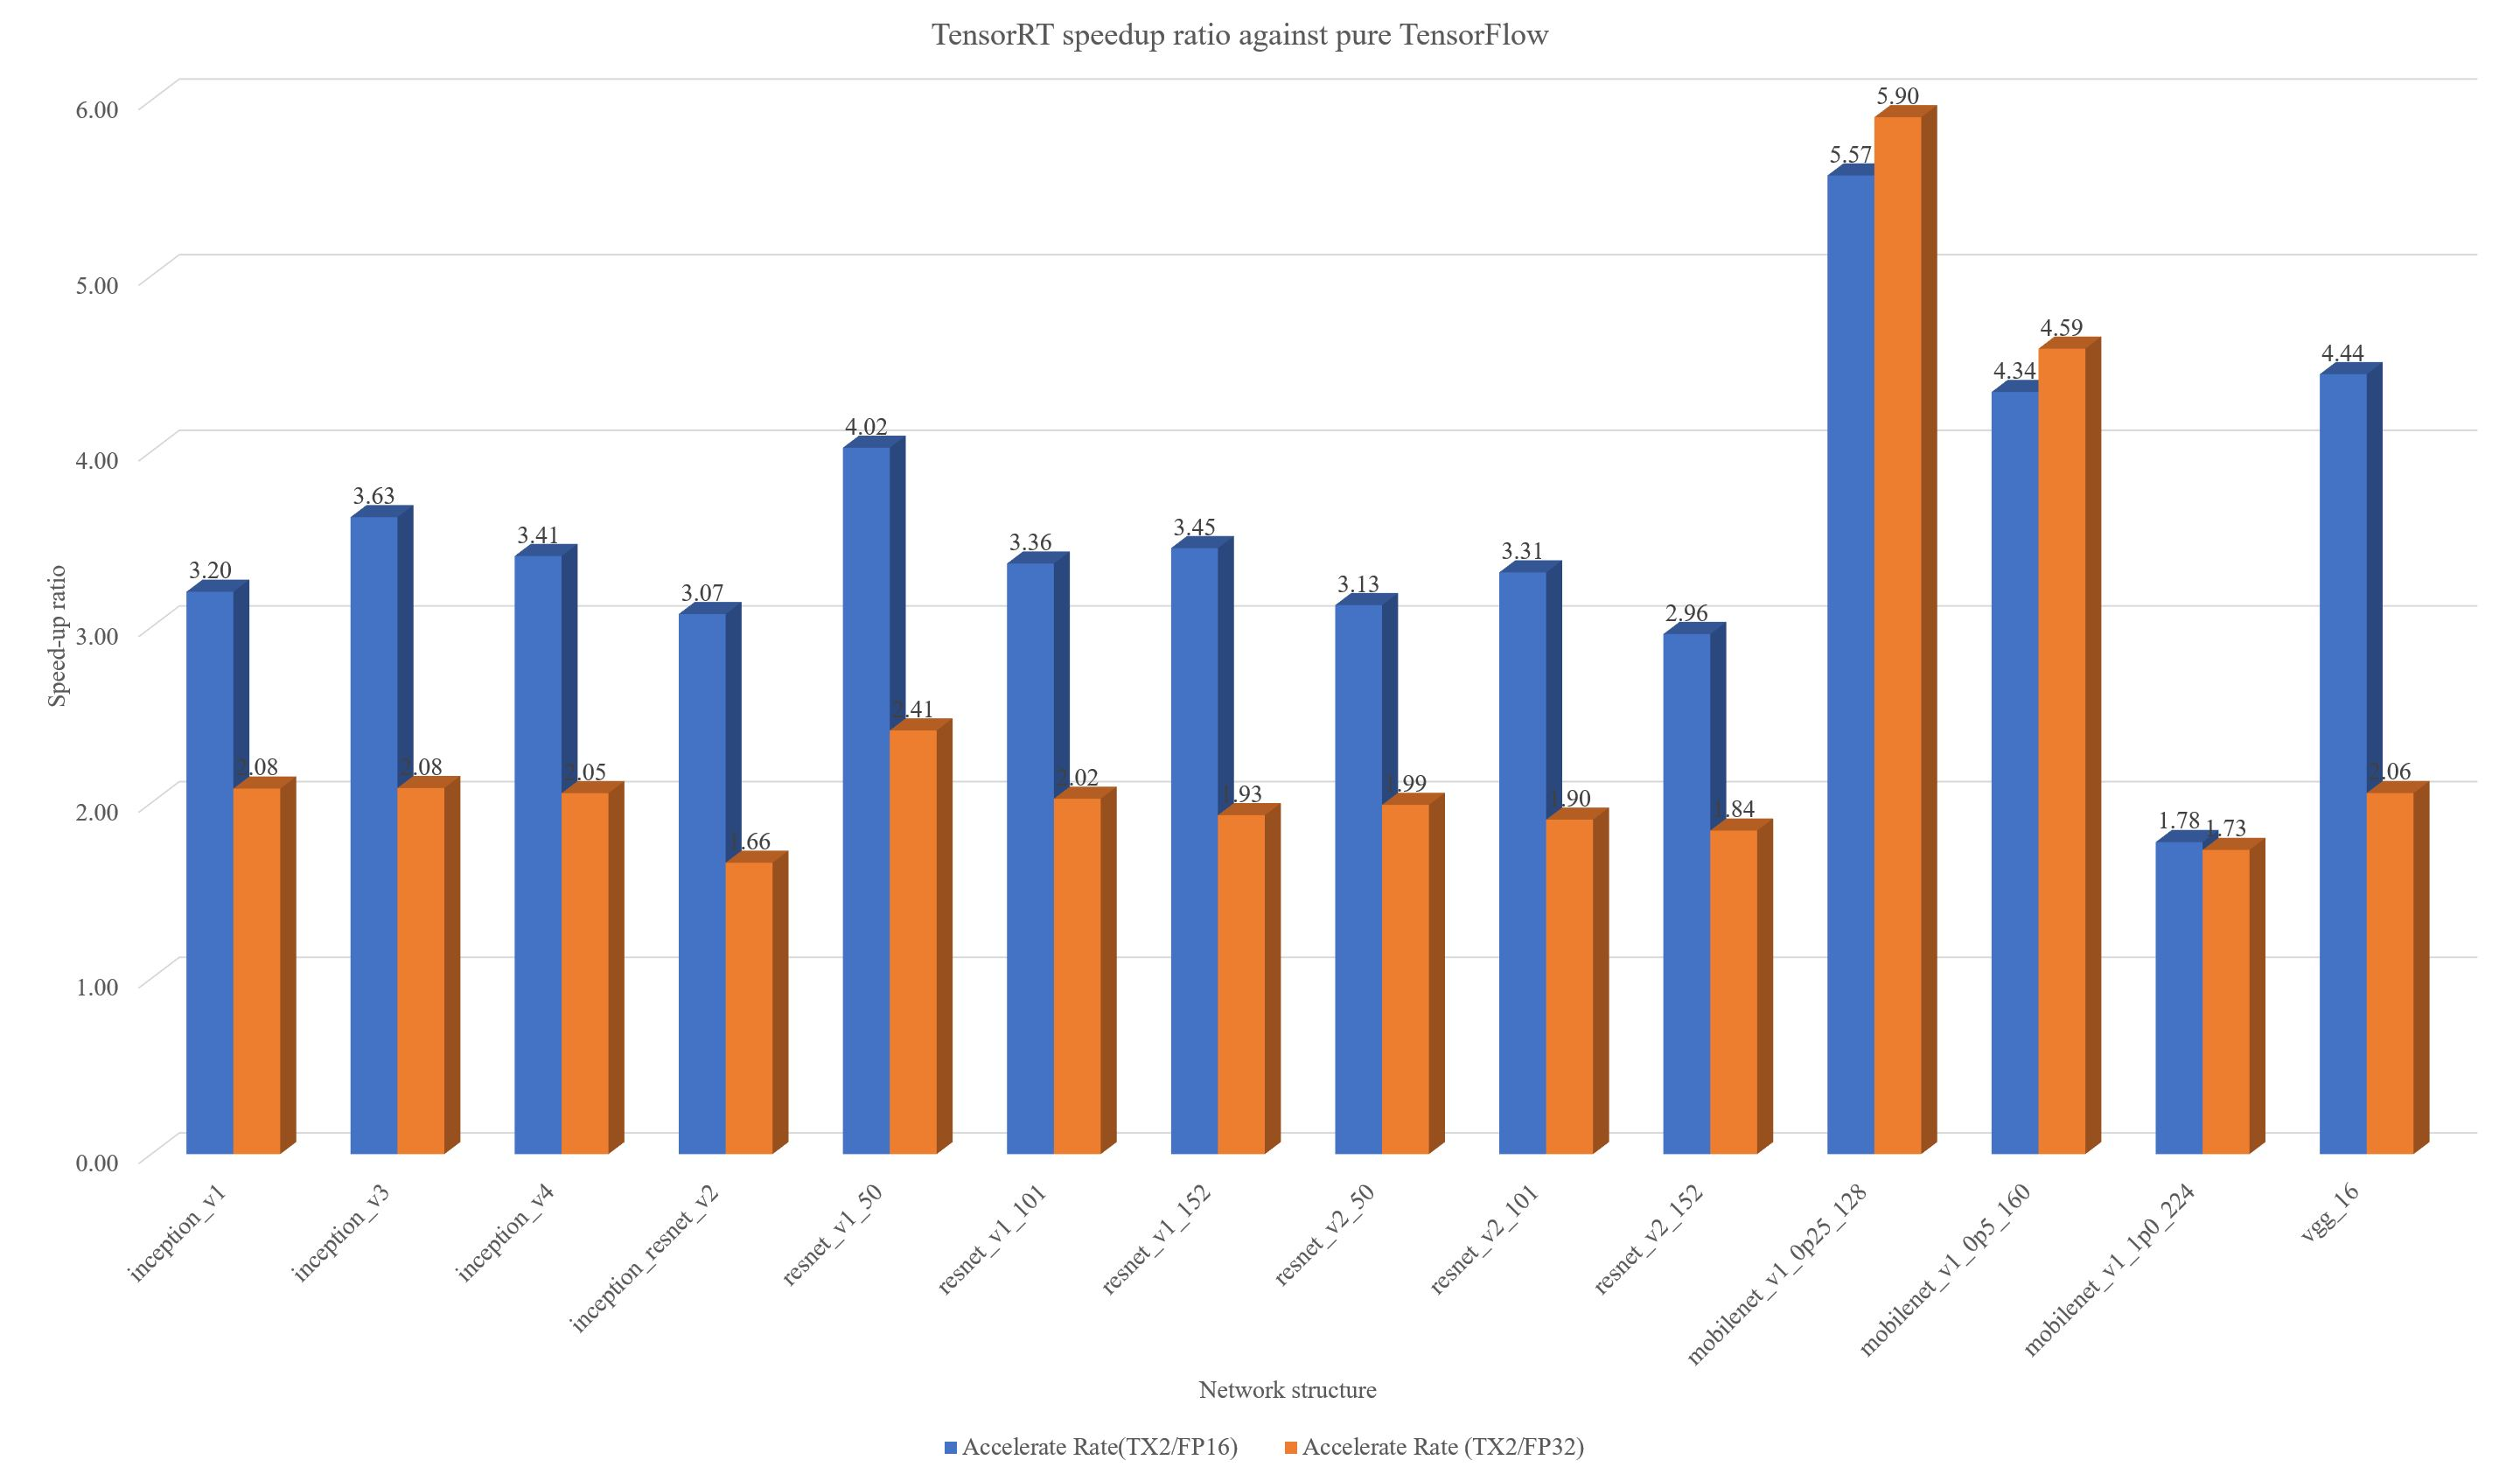
\includegraphics[width=5.5cm]{figures/TENSORRTRATIO.jpg}
			\caption{使用TensorRT优化后的推理延迟及相应加速比}\label{Fig.TENSORRT}
		\end{figure}
		可见结构简单、参数量巨大的vgg\_16采用TensorRT优化后效果较好。而将卷积拆分为逐点和深度的mobileNet由于卷积形状与张量核心不匹配,在半精度下提升比单精度低。然而由于网络本身已经极大压缩,推理速度已经极快。
	\end{frame}
	
	\subsection{Tensor Flow}
	\begin{frame}
		\frametitle{Tensor Flow-GPU::LeNet-5卷积神经网络}
		最后,本文采用最贴近真实应用场景的,基于Tensor Flow框架搭建的LeNet-5,结合上文实验结果进行优化。其中黄色与红色会带来较明显的精度下降,蓝色为原始参数。
		\begin{table}
			\centering
			\caption{基于Tensor Flow框架的CNN的优化结果}
			\begin{tabular}{cccccccc}
				\toprule
				基准时间 &  超参数 &更改方式 &倍率 & 精度 &倍率 & 卷积方式 &倍率 	\\
				\midrule
				54.016(s) & 批大小 & 16 & $ \times17.07 $ & \color[rgb]{0.3,0.4,1.0}{FP32} & \color[rgb]{0.3,0.4,1.0}{$ \times 1 $ } & \color[rgb]{0.3,0.4,1.0}{原始(GEMM)} &\color[rgb]{0.3,0.4,1.0}{$ \times 1 $} \\
				& & 32 & $ \times 5.21 $ & \color[rgb]{0.9,0.7,0.01}{FP16} & \color[rgb]{0.9,0.7,0.01}{$ \times 0.86 $} & 纹理 & $ \times 0.94 $\\
				& & 64 & $ \times 2.10 $ & \color[rgb]{0.9,0.7,0.01}{INT8} & \color[rgb]{0.9,0.7,0.01}{$ \times 0.82 $} & FFT & $ \times 1.11 $\\
				& & \color[rgb]{0.3,0.4,1.0}{128} & \color[rgb]{0.3,0.4,1.0}{$ \times 1 $}& & & & \\
				& & 256 & $ \times 0.51 $ & & & & \\
				& & 512 & $ \times 0.31 $ & & & & \\
				& & \color[rgb]{0.9,0.7,0.01}{1024} & \color[rgb]{0.9,0.7,0.01}{$ \times 0.21 $}& & & & \\
				& 卷积核 & \color[rgb]{0.3,0.4,1.0}{$ 5\times 5 $} & \color[rgb]{0.3,0.4,1.0}{$ \times 1 $} & & & & \\
				& & \color{red}{$ 8\times 8 $} & \color{red}{$ \times 0.97 $} & & & & \\
				\bottomrule
			\end{tabular} \label{table-TFRES} 
		\end{table}
	\end{frame}
	
	\section{总结}
	\begin{frame}
		\frametitle{总结}
		\begin{itemize}
			\item 张量核心在操作数形状、尺寸与硬件参数、调用特征较为匹配的情况下能通过以精度换速度的策略取得较高的性能提升。
			\item 张量核心在图像尺寸较大时进行卷积运算优势明显,而图像尺寸较小时使用纹理内存的直接方法优势明显。
			\item 由于卷积神经网络连接、每层卷积核参数变化较多,故张量核心提升有限。
			\item 使用GPU进行计算时应根据任务特征,如SMO-SVM中的稀疏矩阵优化。
			\item 基于Tensor Flow-GPU框架的应用可以通过调整精度、更改超参数、重写卷积计算方式提升性能。
			\item TensorRT能极大优化训练完毕的网络,为推理带来极大提升。
		\end{itemize}
		截至目前为止,新架构硬件仍然对问题规模、计算方法、数据分布等特征较敏感,实际使用时应根据具体情况权衡。
	\end{frame}

	\section{展望}
	\begin{frame}
		\frametitle{展望}
		\begin{itemize}
			\item 更大规模的矩阵乘加指令
			\item 使用稀疏矩阵优化的矩阵乘加指令
			\item 更细粒度的同步机制
		\end{itemize}
	\end{frame}
\end{document}


